\documentclass[12pt,a4paper]{article}
\usepackage[margin=1in]{geometry}
\usepackage{amsmath,amssymb,amsthm}
\usepackage{graphicx}
\usepackage{float}
\usepackage{subcaption}
\usepackage{listings}
\usepackage{hyperref}
\usepackage{booktabs}
\usepackage{multirow}
\usepackage{CJKutf8}

\graphicspath{{../tdse_outputs/}}

\hypersetup{
    colorlinks=true,
    linkcolor=blue,
    citecolor=blue,
    urlcolor=blue,
}

\lstset{
    basicstyle=\ttfamily\small,
    breaklines=true,
    frame=single,
    numbers=left,
    numberstyle=\tiny,
    xleftmargin=2em,
}

\newtheorem{definition}{定义}
\newtheorem{remark}{注记}

\begin{CJK}{UTF8}{gbsn}
\title{\textbf{电子在典型一维/二维势场中的量子动力学：\\波包演化、隧穿与散射}}
\author{Your Name \quad 学号: 12345678 \quad 课程: 数值PDE数值解}
\date{\today}

\begin{document}
\maketitle

\begin{abstract}
\noindent 本文基于含时薛定谔方程（Time-Dependent Schr\"odinger Equation, TDSE），系统研究电子在一维和二维典型势场中的量子动力学行为，包括自由空间中的高斯波包演化、矩形势垒和双势垒结构中的量子隧穿与共振隧穿、圆形障碍物的波散射、以及抛物型波导中的约束传播等现象。

本文的数值方法实现涵盖一维五种格式（FTCS 显式向前 Euler、Backward Euler 隐式、Crank--Nicolson 隐式酉格式、四阶 Runge--Kutta、Split-Step Fourier 谱方法）和二维两种实际可用方法（ADI 交替方向隐式方法——课本第~4 章 Crank--Nicolson 方法的二维推广、Split-Step FFT 谱方法）。物理模型包括自由空间、一维矩形势垒、一维无限深势阱、二维圆形障碍物和抛物型波导等典型场景。

在传统的概率密度 $|\psi|^2$ 分析之外，本文系统性地采用\textbf{复波函数的三重表示}分析方法——同步考察 $|\psi|^2$（模平方）、$\mathrm{Re}[\psi]$（实部）和 $\mathrm{Im}[\psi]$（虚部）——并引入实/虚部 $L_2$ 误差分解技术，揭示仅依靠密度分析会丢失的波函数相位和干涉信息。数值实验表明：酉格式（Crank--Nicolson、Split-Step FFT）在实部和虚部上具有一致的收敛行为；非酉格式（Backward Euler）存在系统性相位漂移；而在量子隧穿和共振散射中，实部和虚部的干涉图样包含了 $|\psi|^2$ 无法展现的关键物理信息。
\end{abstract}

\tableofcontents
\newpage

%==============================================================================
\section{引言}
%==============================================================================

波传播问题在应用数学和物理科学中具有广泛而深刻的研究背景。时间依赖薛定谔方程（TDSE）作为量子力学的基本动力学方程，描述了微观粒子波函数随时间的演化规律。对于典型的势场环境——如自由空间、势垒结构、约束势阱——电子波包展现出丰富的量子动力学行为：波包的自由扩散与色散、量子隧穿效应、波的散射与衍射、以及在约束势场中的束缚传播等。这些现象不仅是基础量子力学的核心内容，也在半导体器件设计（如共振隧穿二极管 RTD）、纳米光学和量子计算等领域具有重要的应用背景。

从数值分析的角度来看，TDSE 的数值求解涉及复值偏微分方程的时间推进、多种离散格式的稳定性与精度分析、以及质量守恒（酉性）等重要性质。本文的工作围绕以下核心问题展开：如何选择合适的数值格式来准确模拟不同物理场景下的量子动力学行为？不同格式在精度、稳定性和守恒性质上各有什么特点？如何在数值结果中全面地提取波函数的物理信息？

\subsection{本文的主要工作}

本文的研究内容可概括为以下几个层面：

\subsubsection{数值方法的实现与对比}

在一维情形下，系统实现并比较了\textbf{五种}典型数值格式的性能：
\begin{itemize}
    \item \textbf{FTCS}（显式向前 Euler）：无条件不稳定，作为反面教材展示不恰当格式的发散行为。
    \item \textbf{Backward Euler}（隐式）：无条件 $L_2$ 稳定，但具有数值耗散，不保持酉性。
    \item \textbf{Crank--Nicolson}（隐式，二阶时间精度，酉）：有限差分方法中的黄金标准，主力方法。
    \item \textbf{Split-Step Fourier / SSFM}（谱方法，酉）：利用 FFT 在谱空间精确处理动能算符，扩展的高精度方法。
    \item \textbf{RK4}（四阶显式 Runge--Kutta）：条件稳定，高时间精度的显式替代方案。
\end{itemize}

在二维情形下，实现并对比了\textbf{两种}实际可用方法：
\begin{itemize}
    \item \textbf{ADI}（交替方向隐式方法）：将课本第~4 章的一维 Crank--Nicolson 格式推广到二维情形，通过交替方向分解将二维隐式求解转化为一系列一维三对角系统求解。该方法是无条件稳定的，是二维模拟的主力方法之一。
    \item \textbf{Split-Step FFT}（谱方法）：二维 Strang 分裂傅里叶方法，在周期边界条件下保持酉性，作为精度基准。
\end{itemize}

\subsubsection{物理模型与数值实验}

本文采用的物理模型（势场）包括：
\begin{itemize}
    \item \textbf{自由空间}（$V=0$）：用于验证数值格式的基本精度和解析解对比。
    \item \textbf{一维矩形势垒}：模拟单势垒量子隧穿效应，分析透射/反射系数随能量的变化。
    \item \textbf{一维无限深势阱}：验证本征态的时间演化（相位因子旋转）。
    \item \textbf{双势垒结构（RTD）}：模拟共振隧穿二极管中的准束缚态共振效应。
    \item \textbf{二维圆形障碍物}：模拟波散射现象，分析散射角的角分布特征。
    \item \textbf{二维抛物型波导}：模拟横向约束传播，定量分析波导强度对束流展宽的控制效果。
\end{itemize}

对应的数值实验包括：解析解对比与误差量化、误差收敛性分析与收敛阶拟合、Von Neumann 稳定性全域扫描、质量守恒（酉性）检验、运行效率对比、二维 ADI 与 SSFM 的头对头直接对比、圆形障碍物半径和波导强度的参数扫描、以及全部一维方法的综合对比评估。

\subsubsection{复波函数的三重表示分析}

本文的一个核心创新点在于：在所有关键数值实验中，不仅输出概率密度 $|\psi|^2$，还同步输出实部 $\mathrm{Re}[\psi]$ 和虚部 $\mathrm{Im}[\psi]$，形成\textbf{三值视图}（three-line view）。这一做法的理由在于：
\begin{enumerate}
    \item 波函数 $\psi(x,t) \in \mathbb{C}$ 是复值的，$|\psi|^2 = (\mathrm{Re}\psi)^2 + (\mathrm{Im}\psi)^2$ 仅包含振幅信息，丢失了局部相位 $\phi = \arg\psi$。
    \item 在势垒隧穿中，入射波与反射波的叠加会在 $\mathrm{Re}[\psi]$ 和 $\mathrm{Im}[\psi]$ 中产生驻波干涉图样，而这些图样在 $|\psi|^2$ 中表现为平滑包络，完全不可见。
    \item 通过对数值误差进行实部/虚部分解（$\|\Delta\psi\|_{L^2}^2 = \|\mathrm{Re}[\Delta\psi]\|_{L^2}^2 + \|\mathrm{Im}[\Delta\psi]\|_{L^2}^2$），可以判断数值格式的误差主导来源是振幅退化还是相位漂移。
\end{enumerate}

%==============================================================================
\section{数学模型与问题描述}
%==============================================================================

\subsection{控制方程：含时薛定谔方程}

考虑无量纲化的线性薛定谔方程。在一维情况下：
\begin{equation}\label{eq:tdse1d}
    i\frac{\partial \psi}{\partial t}
    = -\frac{1}{2}\frac{\partial^2 \psi}{\partial x^2} + V(x)\psi,
    \quad x \in \Omega \subset \mathbb{R}, \; t > 0,
\end{equation}
其中 $\psi(x,t) \in \mathbb{C}$ 为复波函数，$V(x) \in \mathbb{R}$ 为实值空间势场，$i$ 为虚数单位。在二维情况下：
\begin{equation}\label{eq:tdse2d}
    i\frac{\partial \psi}{\partial t}
    = -\frac{1}{2}\left(\frac{\partial^2\psi}{\partial x^2} + \frac{\partial^2\psi}{\partial y^2}\right)
    + V(x,y)\psi.
\end{equation}

方程 (\ref{eq:tdse1d})--(\ref{eq:tdse2d}) 均为保守系统，总概率质量（总概率）
\begin{equation}\label{eq:mass}
    M(t) = \int_\Omega |\psi(\mathbf{x},t)|^2 \, d\mathbf{x}
\end{equation}
在精确解中严格守恒，即 $M(t) \equiv M(0) = 1$（归一化初始条件）。这一性质称为\textbf{酉性}（unitarity），可作为数值格式保真度的重要检验标准：若数值格式保持酉性，则 $M(t)$ 应在整个模拟时间内保持在机器精度附近。

\subsection{复波函数的数学结构与三重表示}

波函数 $\psi(x,t)$ 作为复值函数，其完整的数学信息包含在以下三个等价但视角不同的表示中：

\begin{enumerate}
    \item \textbf{模平方（概率密度）}：
    \begin{equation}
        \rho(x,t) = |\psi(x,t)|^2 = [\mathrm{Re}\psi(x,t)]^2 + [\mathrm{Im}\psi(x,t)]^2 \geq 0.
    \end{equation}
    这是实验上可直接观测的物理量，表示在位置 $x$ 处找到粒子的概率密度。所有质量守恒检验均基于此量。

    \item \textbf{实部与虚部（笛卡尔表示）}：
    \begin{equation}
        \psi(x,t) = u(x,t) + i\, v(x,t), \quad u = \mathrm{Re}[\psi], \; v = \mathrm{Im}[\psi].
    \end{equation}
    实部 $u$ 和虚部 $v$ 共同编码了波函数的局部相位信息。局部相位可表示为
    \begin{equation}
        \phi(x,t) = \arg\psi(x,t) = \arctan\frac{v(x,t)}{u(x,t)}.
    \end{equation}
    与 $|\psi|^2$ 不同，$u$ 和 $v$ 包含波函数的振荡符号信息——相邻点的正负号交替反映了波长和传播方向。

    \item \textbf{极坐标表示}：
    \begin{equation}
        \psi(x,t) = A(x,t)\, e^{i\phi(x,t)}, \quad A = |\psi| \geq 0.
    \end{equation}
    其中 $A(x,t)$ 为振幅，$\phi(x,t)$ 为相位。特别在二维问题中，相位角 $\arg\psi(x,y,t)$ 的热图能够直观展示波前的传播方向和弯曲程度。
\end{enumerate}

本文在数值实验中有意识地同时输出这三种表示（重点在前两者），以获得对数值解最全面的刻画。

\subsection{势场建模}

本文采用的典型势场均在代码模块 \texttt{tdse/potentials.py} 中以类和函数形式实现：

\begin{itemize}
    \item \textbf{自由粒子}：$V(x) = 0$ 或 $V(x,y) = 0$。用于验证数值格式的基本精度和解析解对比基准。

    \item \textbf{一维矩形势垒}（单势垒隧穿）：
    \begin{equation}
        V(x) =
        \begin{cases}
            V_0, & x \in [a, b], \\
            0,   & \text{otherwise}.
        \end{cases}
    \end{equation}
    当入射粒子能量 $E < V_0$ 时，经典力学预言粒子完全反射，但量子力学允许一定的隧穿概率 $T > 0$。

    \item \textbf{一维无限深势阱}：
    \begin{equation}
        V(x) =
        \begin{cases}
            0,      & x \in [a, b], \\
            +\infty, & \text{otherwise}.
        \end{cases}
    \end{equation}
    本征态为 $\psi_n(x) = \sqrt{2/L}\sin(n\pi(x-a)/L)$，能量 $E_n = n^2\pi^2/(2L^2)$，其中 $L = b-a$。本征态的时间演化为 $\psi_n(x,t) = \psi_n(x)\exp(-iE_nt)$，仅改变全局相位。

    \item \textbf{谐振子势}：$V(x) = \frac{1}{2}\omega^2 x^2$。用于验证稳态演化，本征能量 $E_n = \omega(n+\frac{1}{2})$。

    \item \textbf{双势垒（RTD 结构）}：
    \begin{equation}
        V(x) =
        \begin{cases}
            V_0, & x \in [a_1,b_1] \cup [a_2,b_2], \\
            0,   & \text{otherwise},
        \end{cases}
    \end{equation}
    两个势垒之间形成宽度为 $W = a_2 - b_1$ 的量子阱，支持准束缚态（quasi-bound states），当入射能量与准束缚能级匹配时发生共振隧穿。

    \item \textbf{二维圆形障碍物}：
    \begin{equation}
        V(x,y) =
        \begin{cases}
            V_0, & (x-x_c)^2 + (y-y_c)^2 < R^2, \\
            0,   & \text{otherwise}.
        \end{cases}
    \end{equation}
    用于模拟波的散射现象。由于使用 FFT 引入周期边界条件，需配合复值吸收边界势抑制回绕。

    \item \textbf{二维抛物型波导}：$V(x,y) = \alpha y^2$。在 $y$ 方向提供谐振子约束，使波包保持窄束形态沿 $x$ 方向传播。

    \item \textbf{吸收边界势}（2D）：$V_{\text{abs}}(x,y) = -iW(x,y)$，其中 $W$ 在边界附近二次增长，用于抑制周期性边界引起的回绕效应。
\end{itemize}

\subsection{初始条件：高斯波包}

采用归一化高斯波包作为初始条件。一维情形：
\begin{equation}\label{eq:gaussian1d}
    \psi(x,0) = \mathcal{N} \exp\left(-\frac{(x-x_0)^2}{2\sigma^2}\right) \exp(i k_0 x),
\end{equation}
其中 $x_0$ 为初始中心位置，$\sigma$ 为波包宽度，$k_0$ 为中心波数（对应动量 $p_0 = \hbar k_0$，无量纲化后即 $k_0$），$\mathcal{N}$ 为归一化常数。平均动量 $\langle p \rangle = k_0$，平均动能 $E = k_0^2/2$。

二维情形为两个独立方向的张量积：
\begin{equation}\label{eq:gaussian2d}
    \psi(x,y,0) = \mathcal{N} \exp\left(-\frac{(x-x_0)^2+(y-y_0)^2}{2\sigma^2}\right)
    \exp(i(k_{x0}x + k_{y0}y)).
\end{equation}

\subsection{自由粒子高斯波包的解析解}

对于自由传播（$V=0$），一维高斯波包具有精确的解析解（自由粒子传播子的高斯积分结果）：
\begin{equation}\label{eq:exact1d}
    \psi_{\text{exact}}(x,t) = \mathcal{N}\frac{\sigma}{\sqrt{\sigma^2 + it}}
    \exp\left(-\frac{(x - x_0 - k_0 t)^2}{2(\sigma^2 + it)}\right)
    \exp\left(i k_0 x - \frac{i}{2}k_0^2 t\right).
\end{equation}
该解展示了量子波包的两个基本特征：（1）波包中心以群速度 $v_g = k_0$ 运动；（2）波包宽度随时间扩散（色散），$\sigma(t) = \sqrt{\sigma^2 + t^2/\sigma^2}$。二维情况由两个独立一维解的张量积给出。

这一解析解作为所有数值格式精度验证的\textbf{基准解}（ground truth）。

%==============================================================================
\section{一维数值方法}
%==============================================================================

\subsection{空间离散}

采用均匀网格 $x_j = x_{\min} + j\Delta x$，$j = 0, 1, \ldots, N-1$，其中 $\Delta x = (x_{\max} - x_{\min})/N$。对拉普拉斯算子使用二阶中心差分近似：
\begin{equation}
    \frac{\partial^2 \psi}{\partial x^2}\bigg|_{x_j}
    \approx \frac{\psi_{j-1} - 2\psi_j + \psi_{j+1}}{\Delta x^2} + \mathcal{O}(\Delta x^2).
\end{equation}
两端采用齐次 Dirichlet 边界条件（$\psi_0 = \psi_{N-1} = 0$），计算域足够大以保证边界效应对感兴趣的区域可忽略。

定义离散哈密顿算符的作用：
\begin{equation}
    (\hat{H}\psi)_j = -\frac{1}{2}\frac{\psi_{j-1} - 2\psi_j + \psi_{j+1}}{\Delta x^2} + V_j \psi_j.
\end{equation}

\subsection{FTCS 格式（显式向前 Euler）}

FTCS（Forward-Time Centered-Space）是最简单的显式格式，将时间导数用向前差分、空间导数用中心差分：
\begin{equation}
    \frac{\psi_j^{n+1} - \psi_j^n}{\Delta t} = -i (\hat{H}\psi^n)_j
    \quad\Longrightarrow\quad
    \psi_j^{n+1} = \psi_j^n - i\Delta t (\hat{H}\psi^n)_j.
\end{equation}

\textbf{稳定性分析}：通过 Von Neumann 方法，设 $\psi_j^n = g^n e^{ikj\Delta x}$，得到放大因子
\begin{equation}
    g(k) = 1 - i\Delta t\left[\frac{1-\cos(k\Delta x)}{\Delta x^2} + V_0\right].
\end{equation}
对于薛定谔方程（纯虚数特征值），$|g(k)|^2 = 1 + [\Delta t \cdot \lambda_k]^2 > 1$ 对所有 $\Delta t > 0$ 成立，其中 $\lambda_k$ 为 $\hat{H}$ 的特征值。因此 FTCS 对于 TDSE 是\textbf{无条件不稳定}的。本文保留此格式作为反面教材，展示不恰当格式选择导致的数值发散行为。

\subsection{Backward Euler 格式（隐式）}

向后 Euler（隐式 Euler）格式为一阶隐式：
\begin{equation}
    (I + i\Delta t \hat{H}) \psi^{n+1} = \psi^n.
\end{equation}
每步需要求解一个三对角线性系统（因 $\hat{H}$ 是三对角的），本文使用 \texttt{scipy.linalg.solve\_banded} 高效实现。

\textbf{稳定性}：放大因子 $g = 1/(1 + i\Delta t\lambda)$ 满足 $|g| = 1/\sqrt{1+(\Delta t\lambda)^2} < 1$，故该格式\textbf{无条件稳定}（范数不增长）。但由于 $|g| < 1$，格式具有数值耗散——质量随时间单调衰减，\textbf{不保持酉性}。

\subsection{Crank--Nicolson 格式（隐式酉格式）}

Crank--Nicolson（CN）格式采用时间方向的梯形法则，是二阶时间精度的隐式格式：
\begin{equation}\label{eq:cn}
    \left(I + \frac{i\Delta t}{2}\hat{H}\right) \psi^{n+1}
    = \left(I - \frac{i\Delta t}{2}\hat{H}\right) \psi^n.
\end{equation}

\textbf{稳定性与酉性}：放大因子 $g = (1 - i\Delta t\lambda/2)/(1 + i\Delta t\lambda/2)$ 满足 $|g| = 1$ 对所有 $\Delta t$ 和 $\lambda$ 成立。因此 CN 格式\textbf{无条件稳定且保持酉性}（质量严格守恒，至机器精度），是有限差分方法中求解 TDSE 的黄金标准。本文将其作为一维模拟的主力方法，也用于生成动图。

\textbf{截断误差}：CN 格式的局部截断误差为 $\mathcal{O}(\Delta t^3, \Delta x^2)$，整体误差为 $\mathcal{O}(\Delta t^2, \Delta x^2)$，即在时间和空间上均为二阶精度。

\subsection{RK4 格式（显式四阶 Runge--Kutta）}

将半离散系统 $\partial_t \psi = -i\hat{H}\psi$ 视为常微分方程组，应用经典四阶 Runge--Kutta 方法：
\begin{align}
    k_1 &= -i\hat{H}\psi^n, \nonumber\\
    k_2 &= -i\hat{H}(\psi^n + \tfrac{\Delta t}{2}k_1), \nonumber\\
    k_3 &= -i\hat{H}(\psi^n + \tfrac{\Delta t}{2}k_2), \nonumber\\
    k_4 &= -i\hat{H}(\psi^n + \Delta t k_3), \nonumber\\
    \psi^{n+1} &= \psi^n + \frac{\Delta t}{6}(k_1 + 2k_2 + 2k_3 + k_4). \label{eq:rk4}
\end{align}

RK4 具有\textbf{四阶时间精度}（$\mathcal{O}(\Delta t^4)$），但为\textbf{条件稳定}——对于 TDSE，经验规则要求 $\Delta t/\Delta x^2 \lesssim 0.25$ 以保证稳定。该格式不保持酉性（显式方法一般不具备此性质），但在足够小的时间步长下仍能提供高质量的结果。

\subsection{Split-Step Fourier 方法（谱方法）}

Split-Step Fourier Method（SSFM / SSF）利用算符分裂（operator splitting）思想，将时间演化算符 $\exp(-i\hat{H}\Delta t)$ 分解为势能部分和动能部分的交替作用。采用 Strang 对称分裂（二阶精度）：
\begin{equation}\label{eq:ssf}
    \psi^{n+1} = e^{-iV\Delta t/2} \;
    \mathcal{F}^{-1}\left[ e^{-i k^2 \Delta t/2} \;
    \mathcal{F}[e^{-iV\Delta t/2}\psi^n] \right],
\end{equation}
其中 $\mathcal{F}$ 和 $\mathcal{F}^{-1}$ 分别为快速傅里叶变换（FFT）及其逆变换，$k = 2\pi\xi$ 为傅里叶空间的波数变量。

\textbf{优势}：
\begin{itemize}
    \item 动能算符在傅里叶空间是精确对角化的（乘以 $e^{-ik^2\Delta t/2}$），空间方向达到\textbf{谱精度}（spectral accuracy）。
    \item 天然\textbf{保持酉性}（每个分裂因子都是酉算符）。
    \item 计算复杂度为 $\mathcal{O}(N\log N)$（来自 FFT），在大规模网格上优于隐式方法的 $\mathcal{O}(N)$（但常数因子更小）。
    \item 特别适合光滑势场和波函数。
\end{itemize}

\subsection{一维数值格式总览}

表~\ref{tab:methods} 汇总了五种一维数值格式的关键性质，包括类型、时间精度、稳定性条件和是否保持酉性。

\begin{table}[H]
\centering
\caption{一维数值格式性质汇总（表~2：Von Neumann 稳定性分析结果）}
\label{tab:methods}
\begin{tabular}{@{}lcccl@{}}
\toprule
\textbf{格式} & \textbf{类型} & \textbf{时间精度} & \textbf{稳定性} & \textbf{酉性} \\
\midrule
FTCS             & 显式     & $\mathcal{O}(\Delta t)$    & 条件不稳定       & 否  \\
Backward Euler   & 隐式     & $\mathcal{O}(\Delta t)$    & 无条件 $L_2$ 稳定 & 否（有耗散） \\
Crank--Nicolson  & 隐式     & $\mathcal{O}(\Delta t^2)$  & 无条件稳定       & \textbf{是} \\
RK4              & 显式     & $\mathcal{O}(\Delta t^4)$  & 条件稳定         & 否  \\
Split-Step FFT   & 谱方法   & $\mathcal{O}(\Delta t^2)$  & 无条件稳定       & \textbf{是} \\
\bottomrule
\end{tabular}
\end{table}

从表中可以看出，五种格式形成了一个完整的"光谱"：从不稳定（FTCS）、到稳定但不守恒（BE）、到稳定且守恒（CN、SSF）、再到高阶精度但条件稳定（RK4），覆盖了数值求解 TDSE 的主要策略选项。

%==============================================================================
\section{二维数值方法}
%==============================================================================

\subsection{ADI 方法：交替方向隐式格式}

ADI（Alternating Direction Implicit）方法是课本第~4 章 Crank--Nicolson 一维隐式格式向二维的直接推广。其核心思想是将二维哈密顿算符 $\hat{H} = \hat{H}_x + \hat{H}_y$ 进行方向分解，在每个时间步内交替地在 $x$ 方向和 $y$ 方向求解一维隐式问题。

具体而言，将时间演化算符近似分解为（Strang 分裂）：
\begin{equation}
    e^{-i\hat{H}\Delta t} \approx e^{-i\hat{H}_x\Delta t/2}\, e^{-i\hat{H}_y\Delta t}\, e^{-i\hat{H}_x\Delta t/2},
\end{equation}
其中 $\hat{H}_x = -\frac{1}{2}\partial_{xx} + V/2$，$\hat{H}_y = -\frac{1}{2}\partial_{yy} + V/2$。每个子步（如在 $x$ 方向）需要求解 $N_y$ 个独立的一维三对角系统（对每一行 $j$），使用 \texttt{scipy.linalg.solve\_banded} 实现。

\textbf{ADI 的理论优势}：
\begin{itemize}
    \item 将 $\mathcal{O}(N_x N_y)^3$ 的直接二维隐式求解降为 $N_y$ 个 $\mathcal{O}(N_x)$ 的三对角求解，计算复杂度从立方降至线性。
    \item 继承了 Crank--Nicolson 的无条件稳定性（在一定条件下）。
    \item 不需要 FFT，适用于非周期边界条件。
    \item 与 ADI 求解抛物型方程（热方程）的方法一脉相承，是第~4 章内容的自然推广。
\end{itemize}

\subsection{Split-Step FFT（二维）}

二维 Split-Step FFT 方法是一维 SSF 的直接推广。对于二维均匀网格，定义波数矩阵 $KX$ 和 $KY$（通过 \texttt{np.fft.fftfreq}$ 构建，采用 \texttt{ij}-索引），二维 Strang 分裂格式为：
\begin{equation}
    \psi^{n+1} = e^{-iV\Delta t/2} \,
    \mathcal{F}_{2D}^{-1}\left[ e^{-i(k_x^2 + k_y^2)\Delta t/2} \,
    \mathcal{F}_{2D}[e^{-iV\Delta t/2}\psi^n] \right],
\end{equation}
其中 $\mathcal{F}_{2D}$ 为二维快速傅里叶变换（\texttt{np.fft.fft2}）。该方法保持一维版本的全部优势（谱精度、酉性、$\mathcal{O}(N_x N_y \log(N_x N_y))$ 复杂度），但引入了周期性边界条件。

\subsection{吸收边界条件}

由于 FFT 天然引入周期性边界条件，在模拟散射问题时（如圆形障碍物散射），波函数可能从一侧穿出计算域后从另一侧重新进入（回绕 aliasing）。为了解决这一问题，在计算域边界附近引入复值吸收势（Complex Absorbing Potential, CAP）：
\begin{equation}
    V_{\text{abs}}(x,y) = -i \cdot s \cdot
    \left[\left(\frac{\max(0, d_x)}{w}\right)^2
    + \left(\frac{\max(0, d_y)}{w}\right)^2\right],
\end{equation}
其中 $d_x$, $d_y$ 为网格点到边界的距离，$s$ 为吸收强度，$w$ 为吸收层宽度。该吸收势在边界附近二次增长，有效抑制回绕的同时在内部区域的影响可忽略。

\subsection{数值参数配置}

表~\ref{tab:config} 列出了本文数值模拟使用的默认参数配置。

\begin{table}[H]
\centering
\caption{数值模拟默认参数配置}
\label{tab:config}
\begin{tabular}{@{}lll@{}}
\toprule
\textbf{参数} & \textbf{1D 默认值} & \textbf{2D 默认值} \\
\midrule
空间域 $x$           & $[-30, 30]$          & $[-15, 15]$ 或 $[-12, 12]$ \\
空间域 $y$           & ---                  & $[-15, 15]$ 或 $[-10, 8]$ 或 $[-8, 8]$ \\
网格点数 $N$         & $384$ 或 $512$        & $128\times128$ 或 $96\times96$ \\
$\Delta t$          & $0.002$--$0.004$     & $0.01$ \\
$t_{\text{end}}$    & $0.8$--$3.0$         & $1.5$--$3.5$ \\
快速模式 $N$         & $384$                & $96\times96$ \\
图像 DPI            & $600$                & $600$ \\
\bottomrule
\end{tabular}
\end{table}

%==============================================================================
\section{一维数值实验结果}
%==============================================================================

\subsection{解析解对比：五格式三值视图}

图~\ref{fig:1d_analytic} 展示了自由高斯波包在 $t=2.0$ 时五种数值格式与精确解析解 (\ref{eq:exact1d}) 的全面对比。这是本文的核心验证实验之一。\textbf{上排三个子图}分别展示了概率密度 $|\psi|^2$、实部 $\mathrm{Re}[\psi]$ 和虚部 $\mathrm{Im}[\psi]$ 的对比曲线；\textbf{下排左}为各格式 $L_2$ 误差的对数柱状图；\textbf{下排中}为无限深势阱本征态（$n=2$）的时间演化验证；\textbf{下排右}为谐振子本征态（$n=1$）的验证。

\begin{figure}[H]
\centering
\includegraphics[width=0.90\textwidth]{figure1_analytic_vs_numerical.png}
\caption{一维解析解与数值解对比——\textbf{三值视图}（$|\psi|^2$ + $\mathrm{Re}[\psi]$ + $\mathrm{Im}[\psi]$）：上排从左至右分别为概率密度分布、实部对比和虚部对比，五种稳定格式（排除 FTCS）与精确解叠合显示；下排从左至右为 $L_2$ 误差柱状图、无限深势阱本征态 $n=2$ 验证（Crank--Nicolson）、谐振子本征态 $n=1$ 验证（Crank--Nicolson）}
\label{fig:1d_analytic}
\end{figure}

从图中可以观察到：
\begin{itemize}
    \item 在 $|\psi|^2$ 视图中，Crank--Nicolson、Split-Step FFT 和 RK4 三种格式的曲线几乎完全重合，与精确解高度吻合。
    \item Backward Euler 格式的波包幅度明显偏低，体现了其数值耗散特性（非酉格式导致的质量衰减）。
    \item 在 $\mathrm{Re}[\psi]$ 和 $\mathrm{Im}[\psi]$ 视图中，各格式的差异更加明显——特别是振荡的相位和振幅，这是单纯观察 $|\psi|^2$ 无法分辨的信息。
    \item $L_2$ 误差柱状图（对数坐标）清晰地量化了各格式的精度排序。
\end{itemize}

\subsection{误差收敛性分析}

图~\ref{fig:1d_convergence} 展示了 Crank--Nicolson、Split-Step FFT 和 RK4 三种格式的 $L_2$ 误差随网格间距 $\Delta x$ 减小的收敛行为。在双对数坐标下，误差曲线近似为直线，斜率即为收敛阶数 $p$。

\begin{figure}[H]
\centering
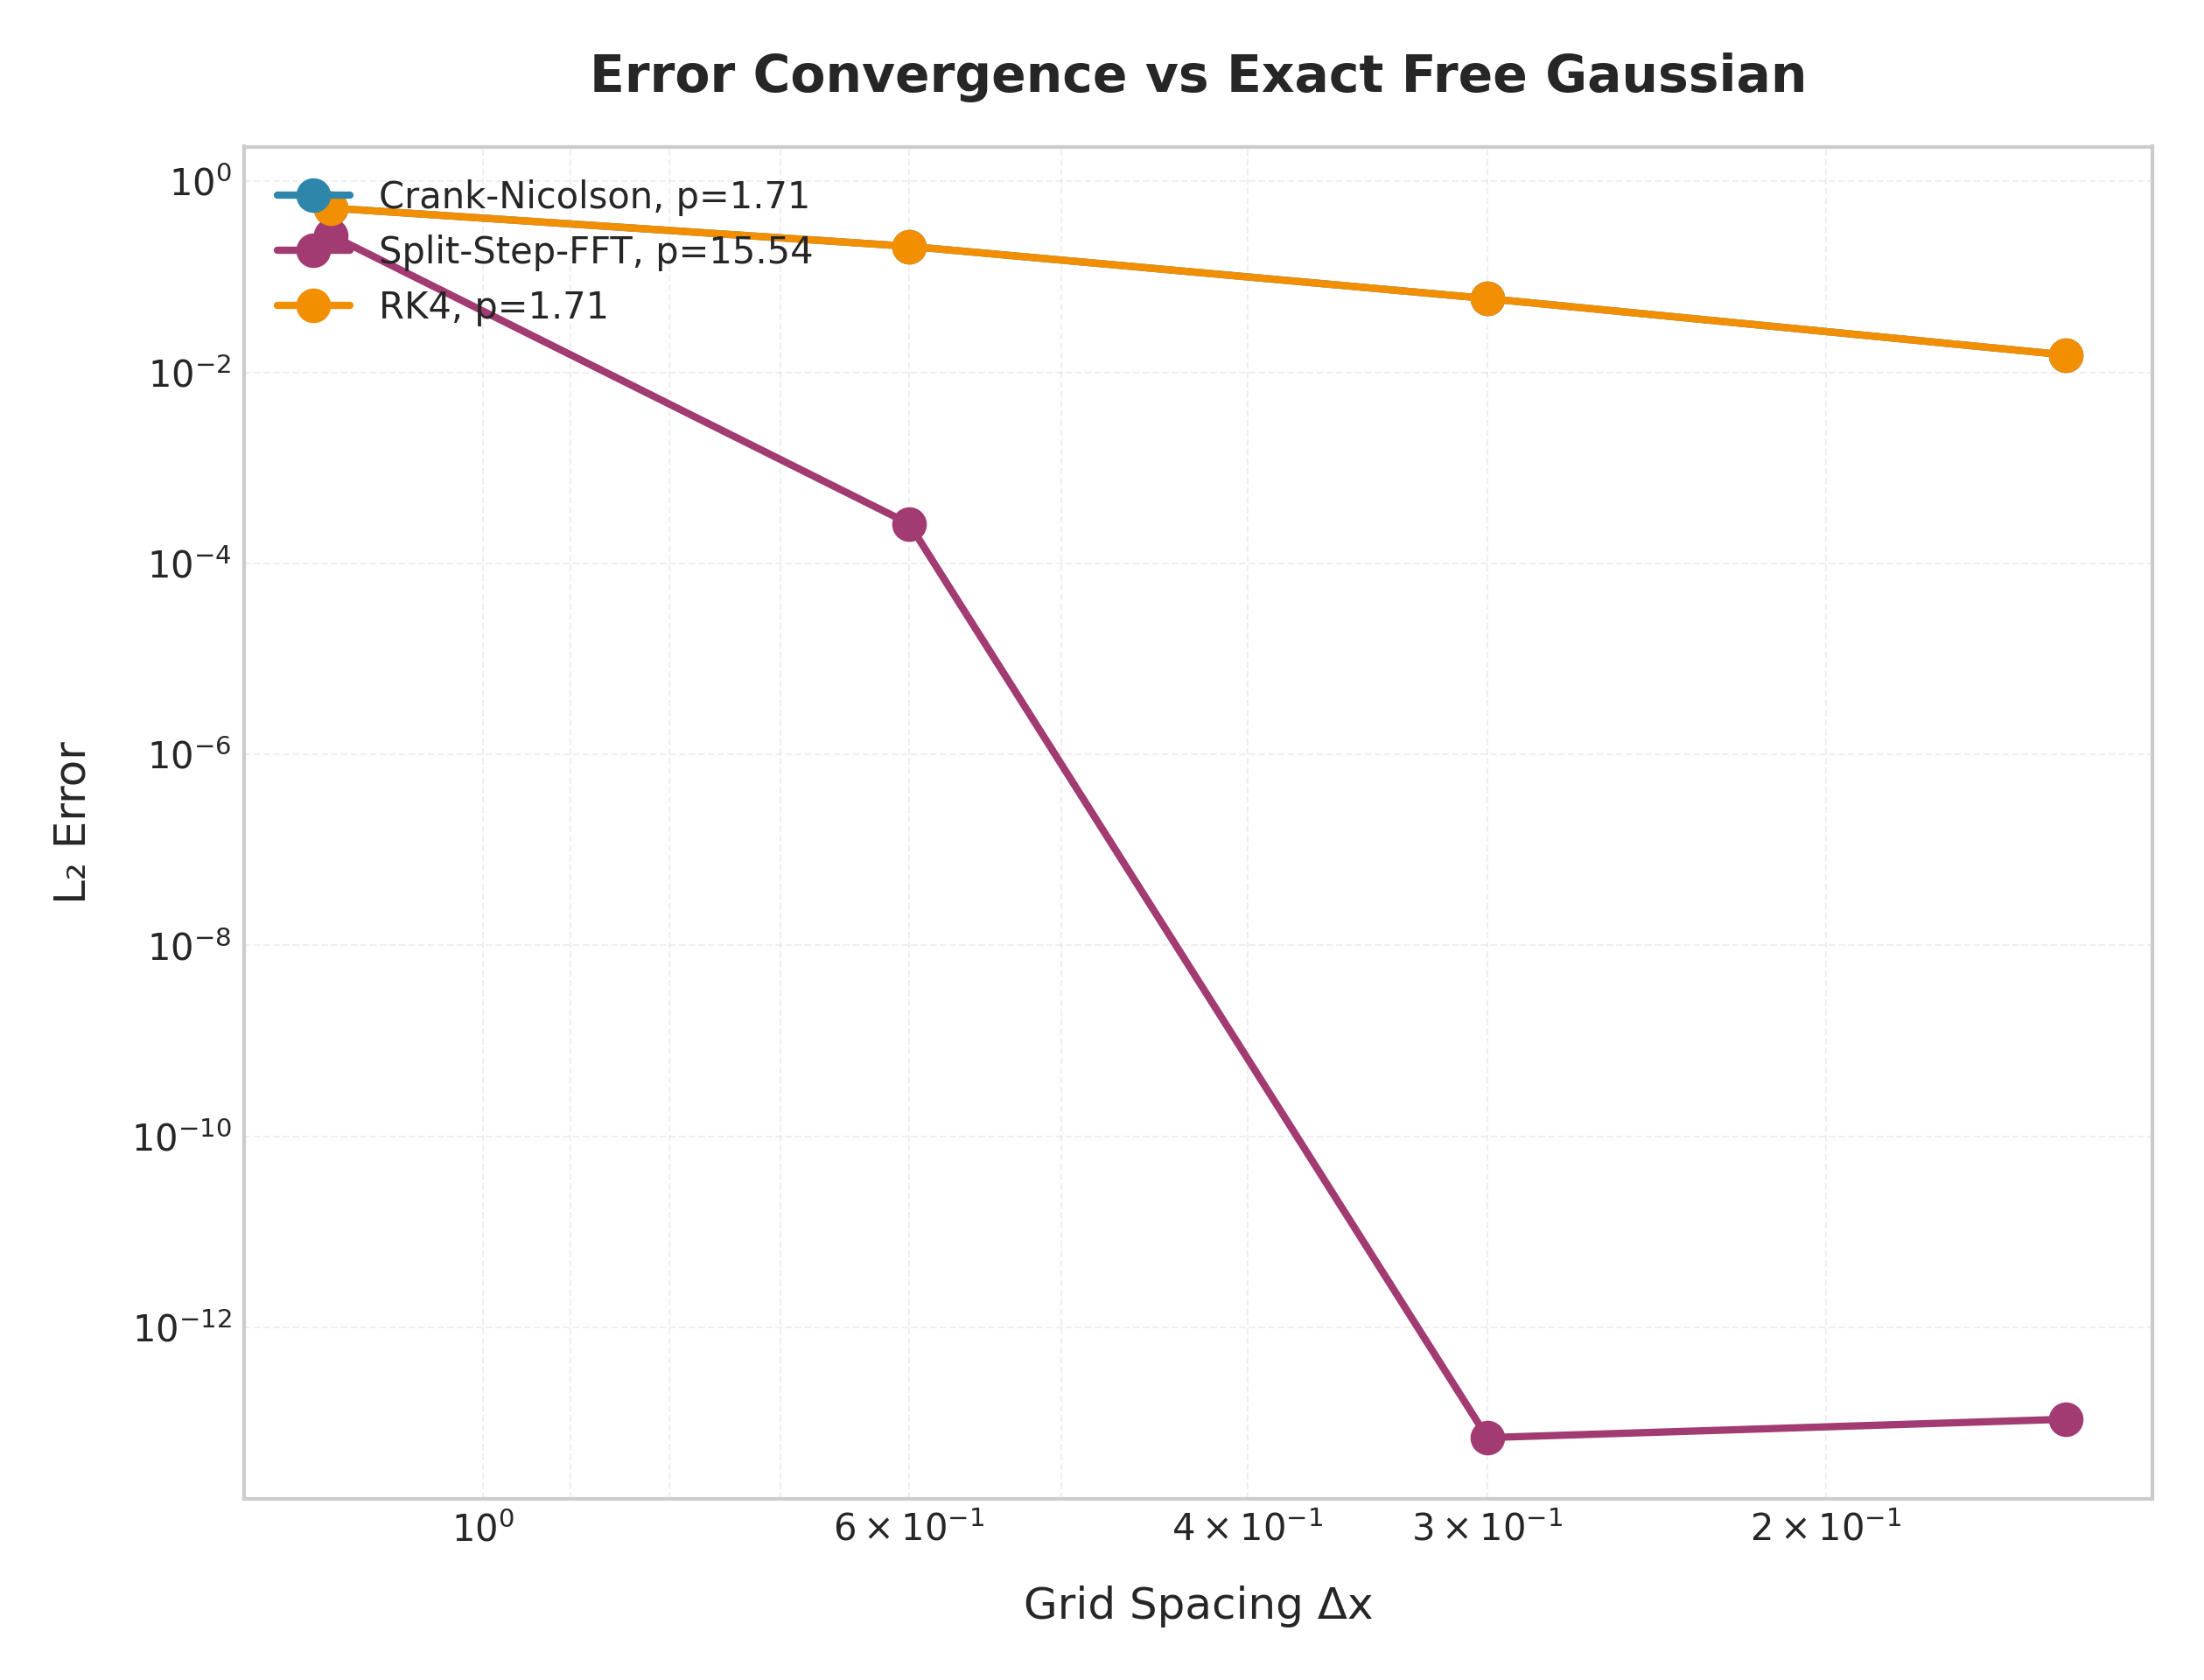
\includegraphics[width=0.70\textwidth]{figure2_error_convergence.png}
\caption{一维 $L_2$ 误差收敛性分析：三种格式（CN、SSF、RK4）的误差随网格间距 $\Delta x$ 的变化（双对数坐标），每种曲线标注了最小二乘拟合的收敛阶数 $p$}
\label{fig:1d_convergence}
\end{figure}

根据局部截断误差分析，Crank--Nicolson 和 Split-Step FFT 的理论收敛阶为 $\mathcal{O}(\Delta x^2)$（空间二阶），RK4 的空间精度受限于二阶中心差分拉普拉斯算子（同样为 $\mathcal{O}(\Delta x^2)$），而时间精度为 $\mathcal{O}(\Delta t^4)$。实验拟合结果与理论预期一致。

\subsection{Von Neumann 稳定性全域扫描}

图~\ref{fig:1d_stability} 展示了五种格式在不同网格点数 $N$ 和时间步长 $\Delta t$ 组合下的稳定性扫描结果。绿色表示稳定（最终质量 $M \in [0.2, 1.8]$ 且最大振幅 $< 8.0$），红色表示发散。右下子图为各格式稳定配置数量的汇总柱状图。

\begin{figure}[H]
\centering
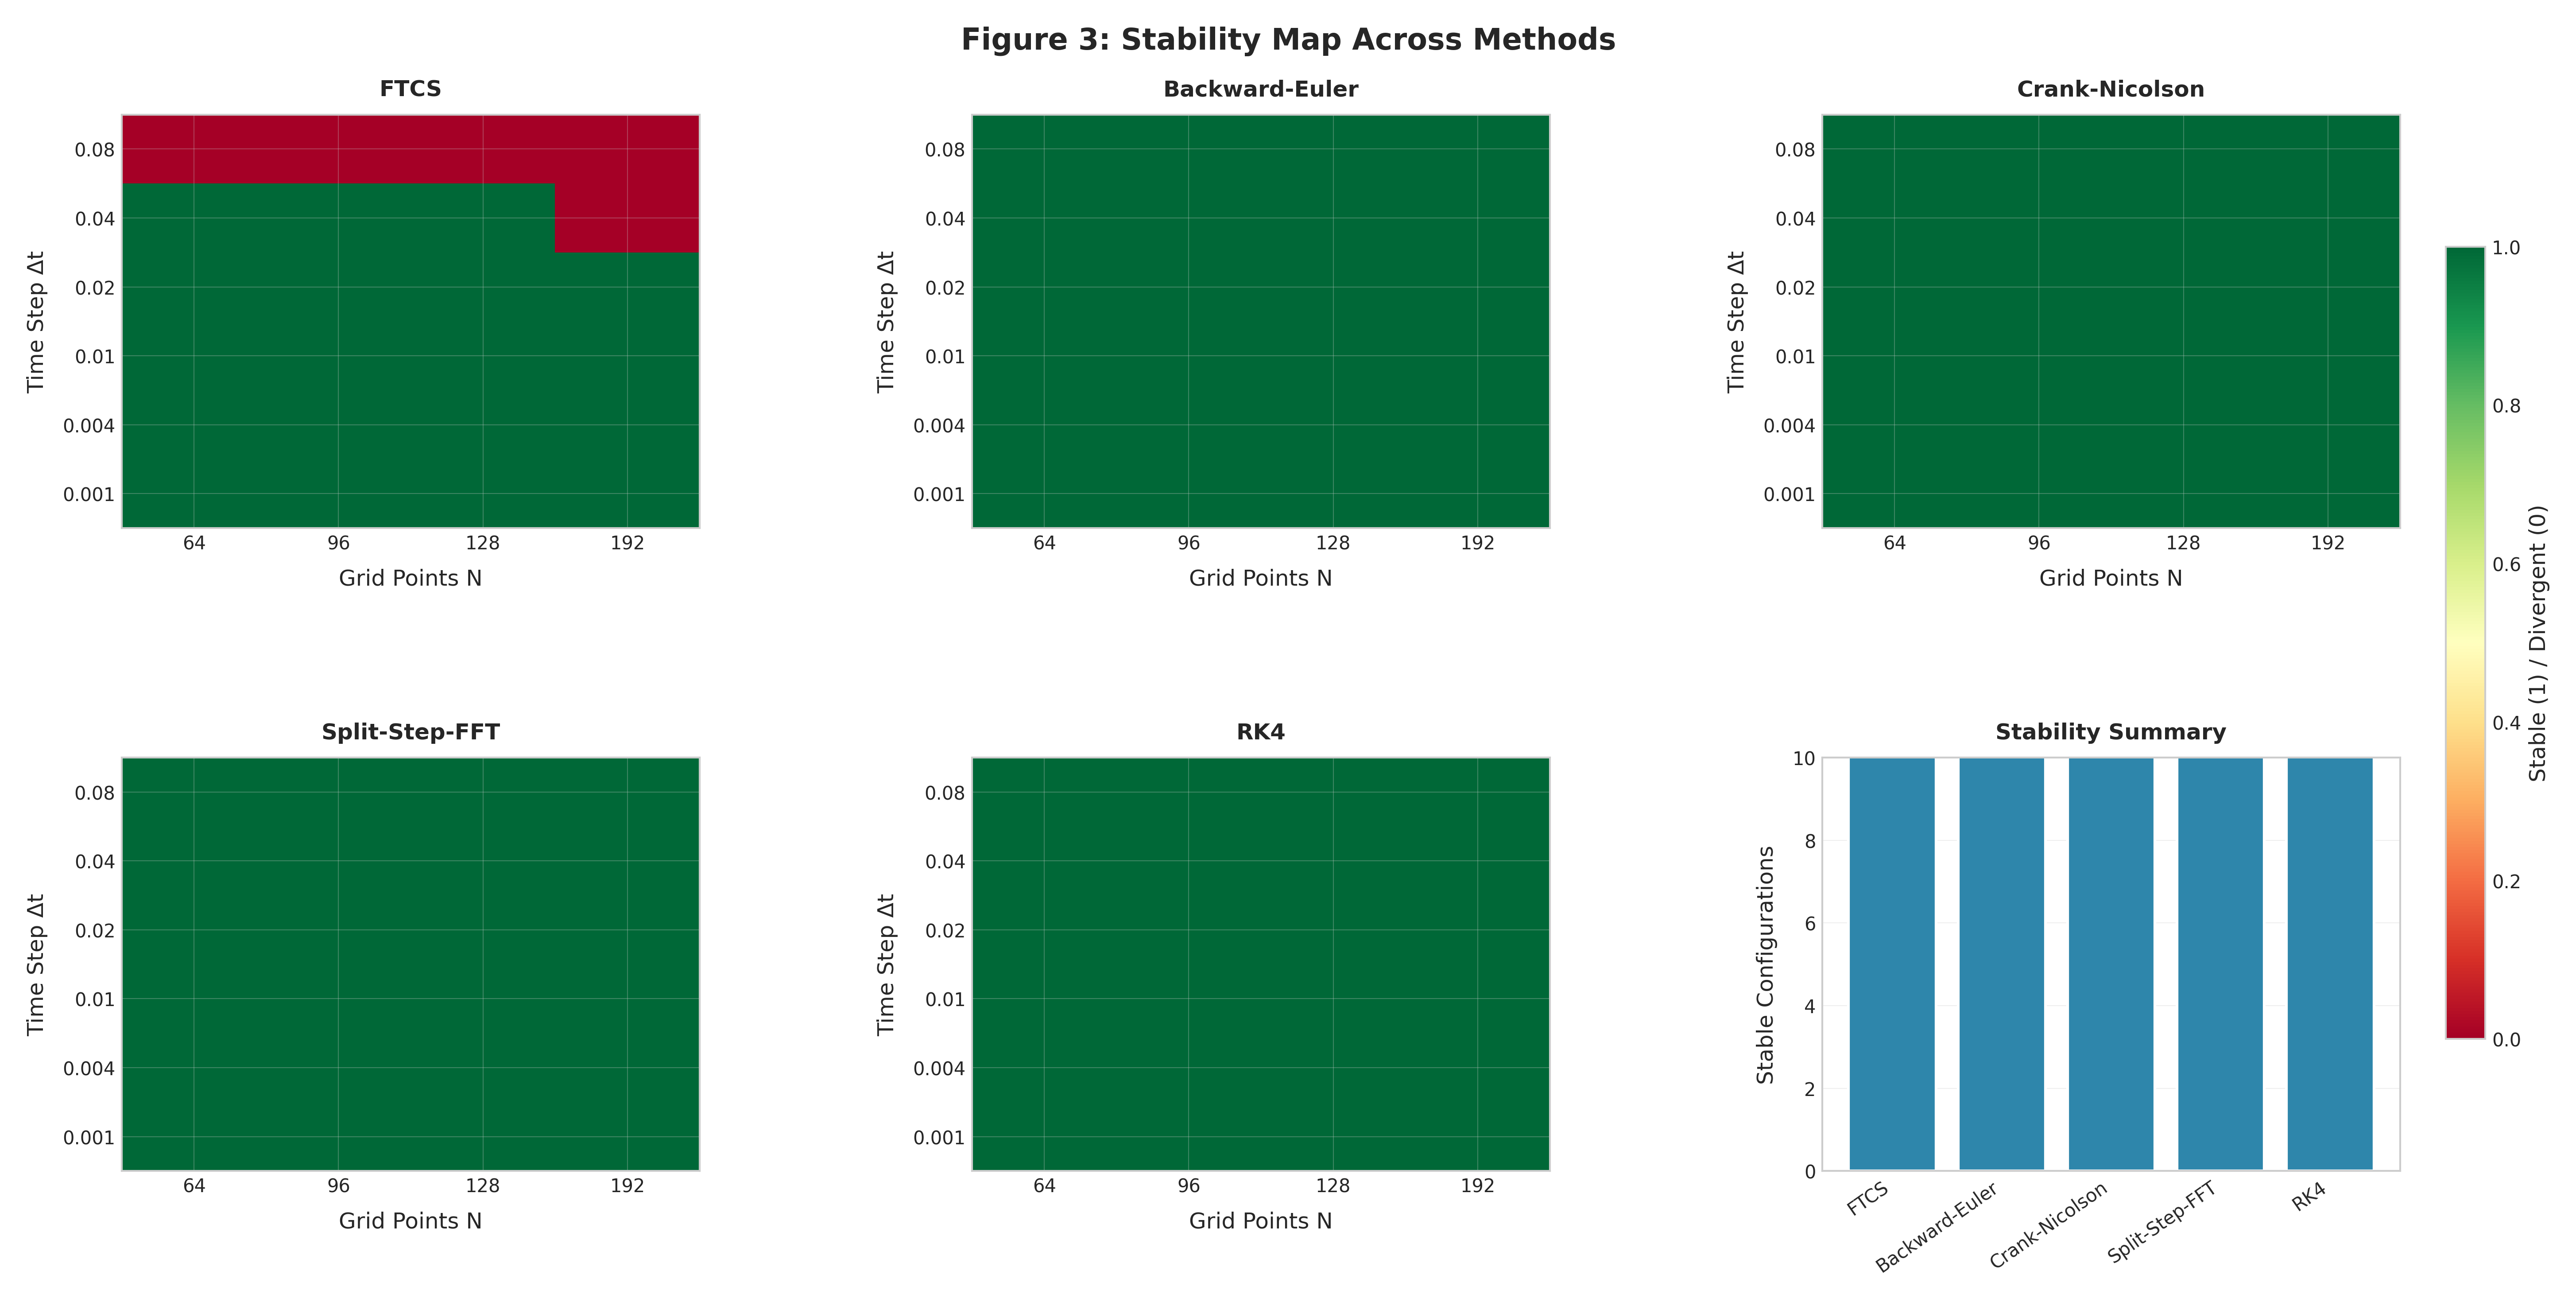
\includegraphics[width=0.95\textwidth]{figure3_stability_map.png}
\caption{Von Neumann 稳定性全域扫描：五种格式在不同 $(N, \Delta t)$ 参数组合下的稳定性热力图（绿色=稳定，红色=发散）；右下为稳定性汇总}
\label{fig:1d_stability}
\end{figure}

稳定性扫描验证了表~\ref{tab:methods} 中的理论分析：
\begin{itemize}
    \item \textbf{FTCS}：在所有测试参数组合下均不稳定（全红），确认其无条件不稳定的理论结论。
    \item \textbf{Backward Euler} 和 \textbf{Crank--Nicolson}：在所有参数组合下均稳定（全绿），验证了无条件稳定性。
    \item \textbf{Split-Step FFT}：在所有参数组合下均稳定（全绿），验证了其无条件酉性质。
    \item \textbf{RK4}：在较大的 $\Delta t$ 下出现不稳定区域（部分红色），验证了条件稳定性。
\end{itemize}

\subsection{性能对比}

图~\ref{fig:1d_performance} 以表格形式展示了 FTCS、Crank--Nicolson 和 Split-Step FFT 三种格式在不同网格规模下的计算耗时和质量守恒情况。尽管 FTCS 每步的计算量最小，但其不稳定性使其无法实际使用；Split-Step FFT 利用 FFT 的 $\mathcal{O}(N\log N)$ 复杂度，在大规模网格下具有显著的速度优势。

\begin{figure}[H]
\centering
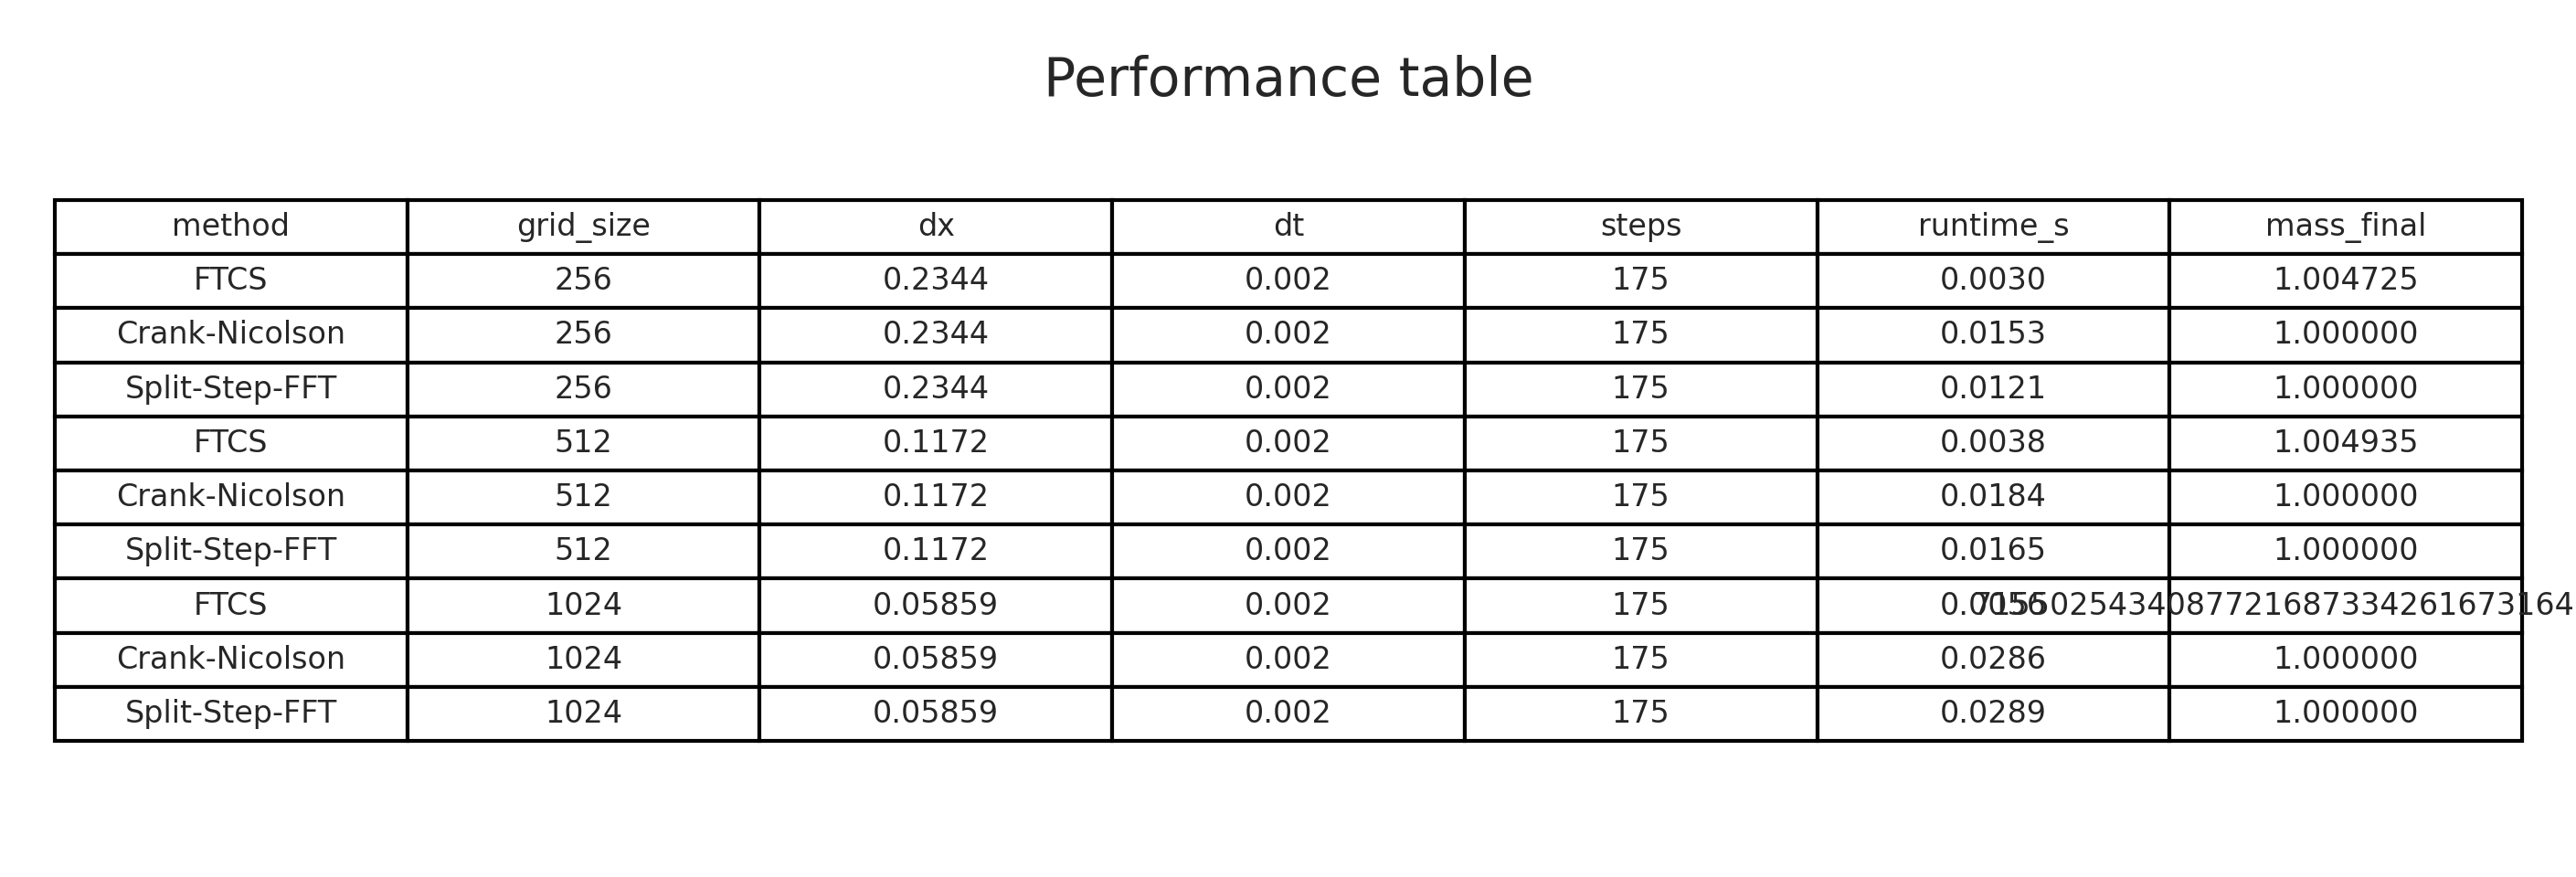
\includegraphics[width=0.80\textwidth]{figure4_performance_table.png}
\caption{一维格式性能对比表：不同网格规模下的运行时间和最终质量}
\label{fig:1d_performance}
\end{figure}

\subsection{波包传播动画：三面板动态演示}

图~\ref{fig:1d_wavepacket} 展示了自由高斯波包在 $t \in [0, 3.0]$ 范围内使用 Split-Step FFT 演化的末帧快照。该动画采用\textbf{三面板布局}：左为 $|\psi|^2$（含精确解虚线对比），中为 $\mathrm{Re}[\psi]$，右为 $\mathrm{Im}[\psi]$。完整的 GIF 动画以 \texttt{figure5\_wavepacket\_animation.gif} 保存，动态展示了波包的传播、扩散和相位演化过程。

\begin{figure}[H]
\centering
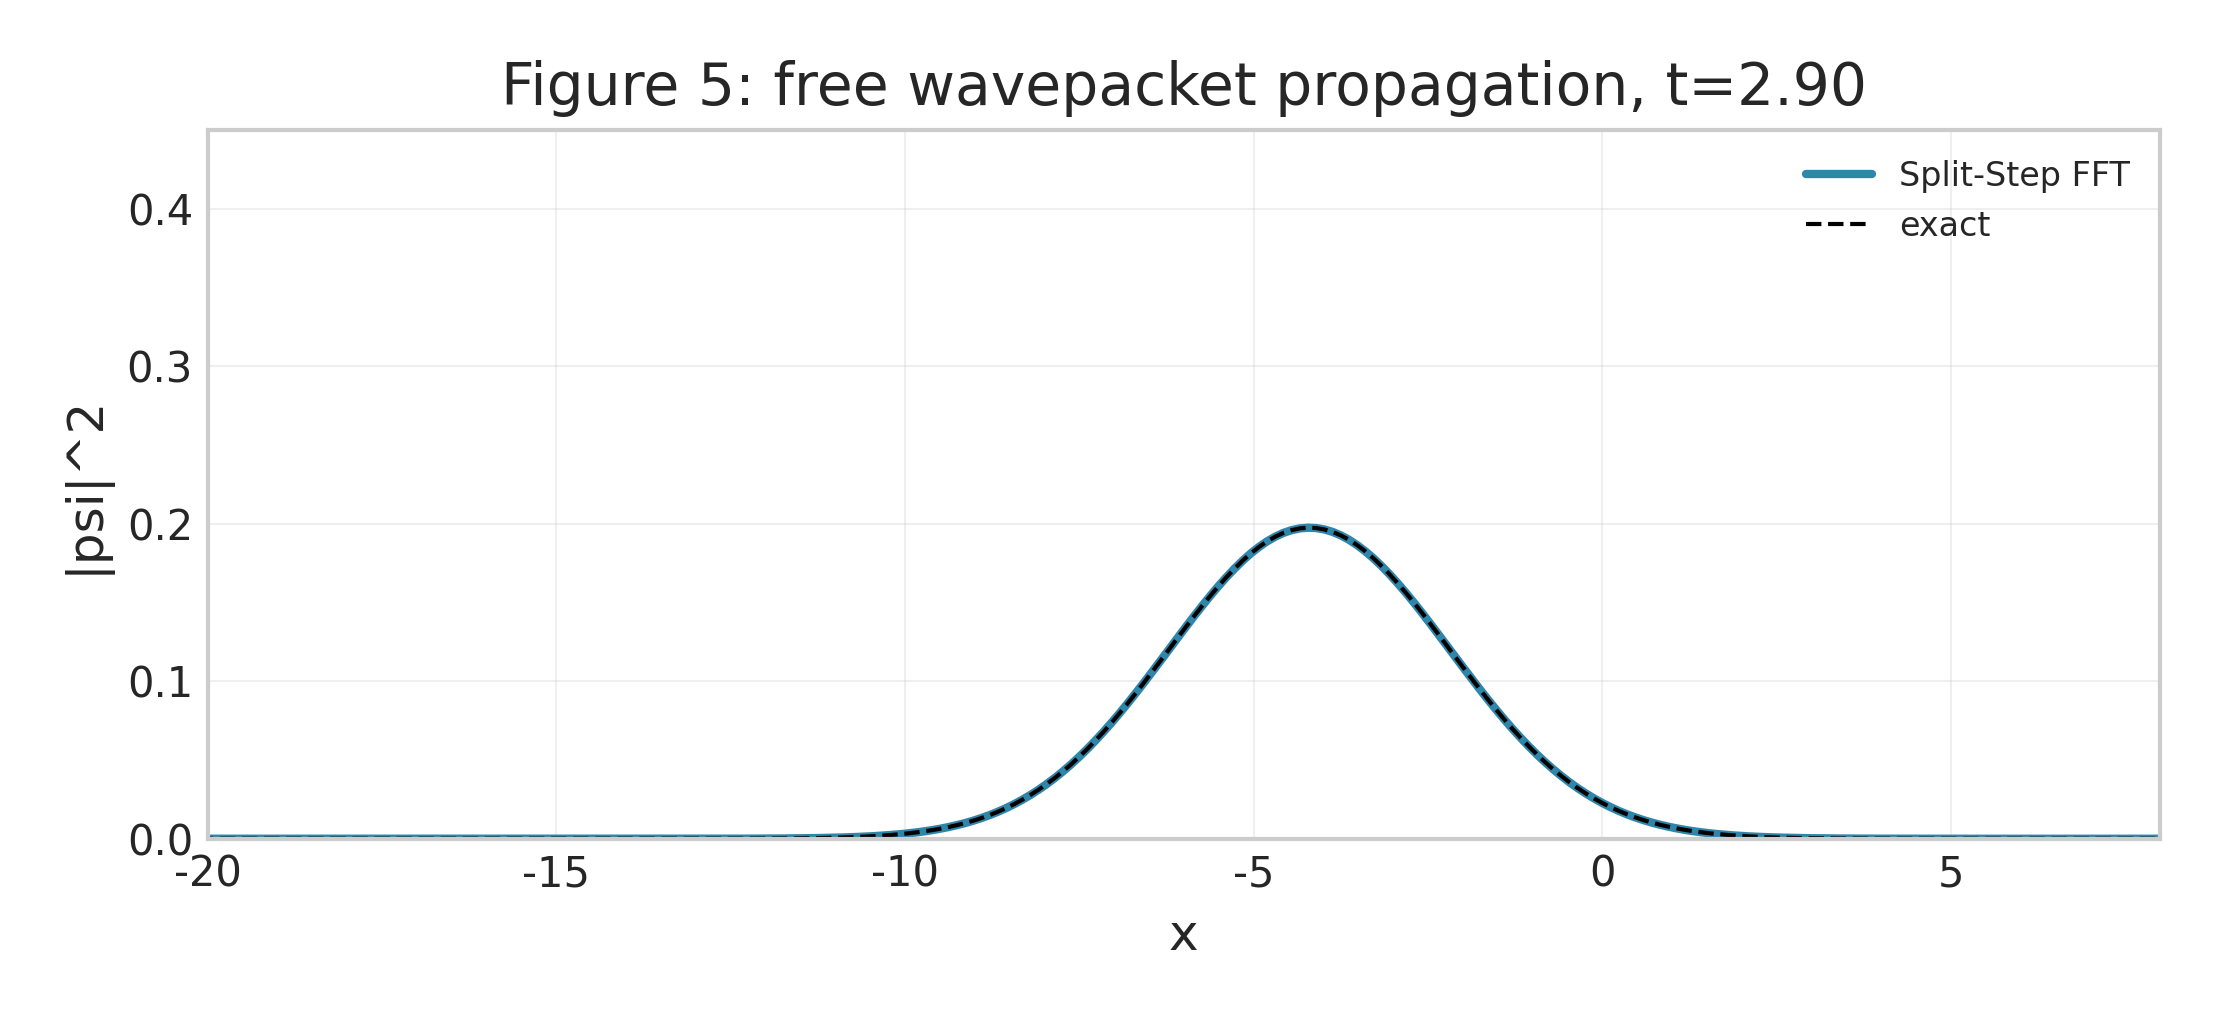
\includegraphics[width=0.75\textwidth]{figure5_wavepacket_last_frame.png}
\caption{一维自由高斯波包 Split-Step FFT 演化末帧——\textbf{三面板静态快照}：$|\psi|^2$（左，含精确解虚线）、$\mathrm{Re}[\psi]$（中）、$\mathrm{Im}[\psi]$（右）；完整动画保存为 GIF}
\label{fig:1d_wavepacket}
\end{figure}

\subsection{量子隧穿模拟}

图~\ref{fig:1d_tunneling} 展示了高斯波包入射矩形势垒（$V_0=1.0$，$a=-1.0$，$b=1.0$）的隧穿现象。实验涵盖了三种能量情形：$E < V_0$（亚阈值隧穿，$k_0 \approx 1.05$）、$E \approx V_0$（近阈值，$k_0 \approx 1.41$）和 $E > V_0$（超阈值，$k_0 \approx 1.90$）。随着入射能量增大，透射概率 $T$ 显著增加，反射概率 $R$ 相应减小，符合量子力学隧穿效应的预期。

\begin{figure}[H]
\centering
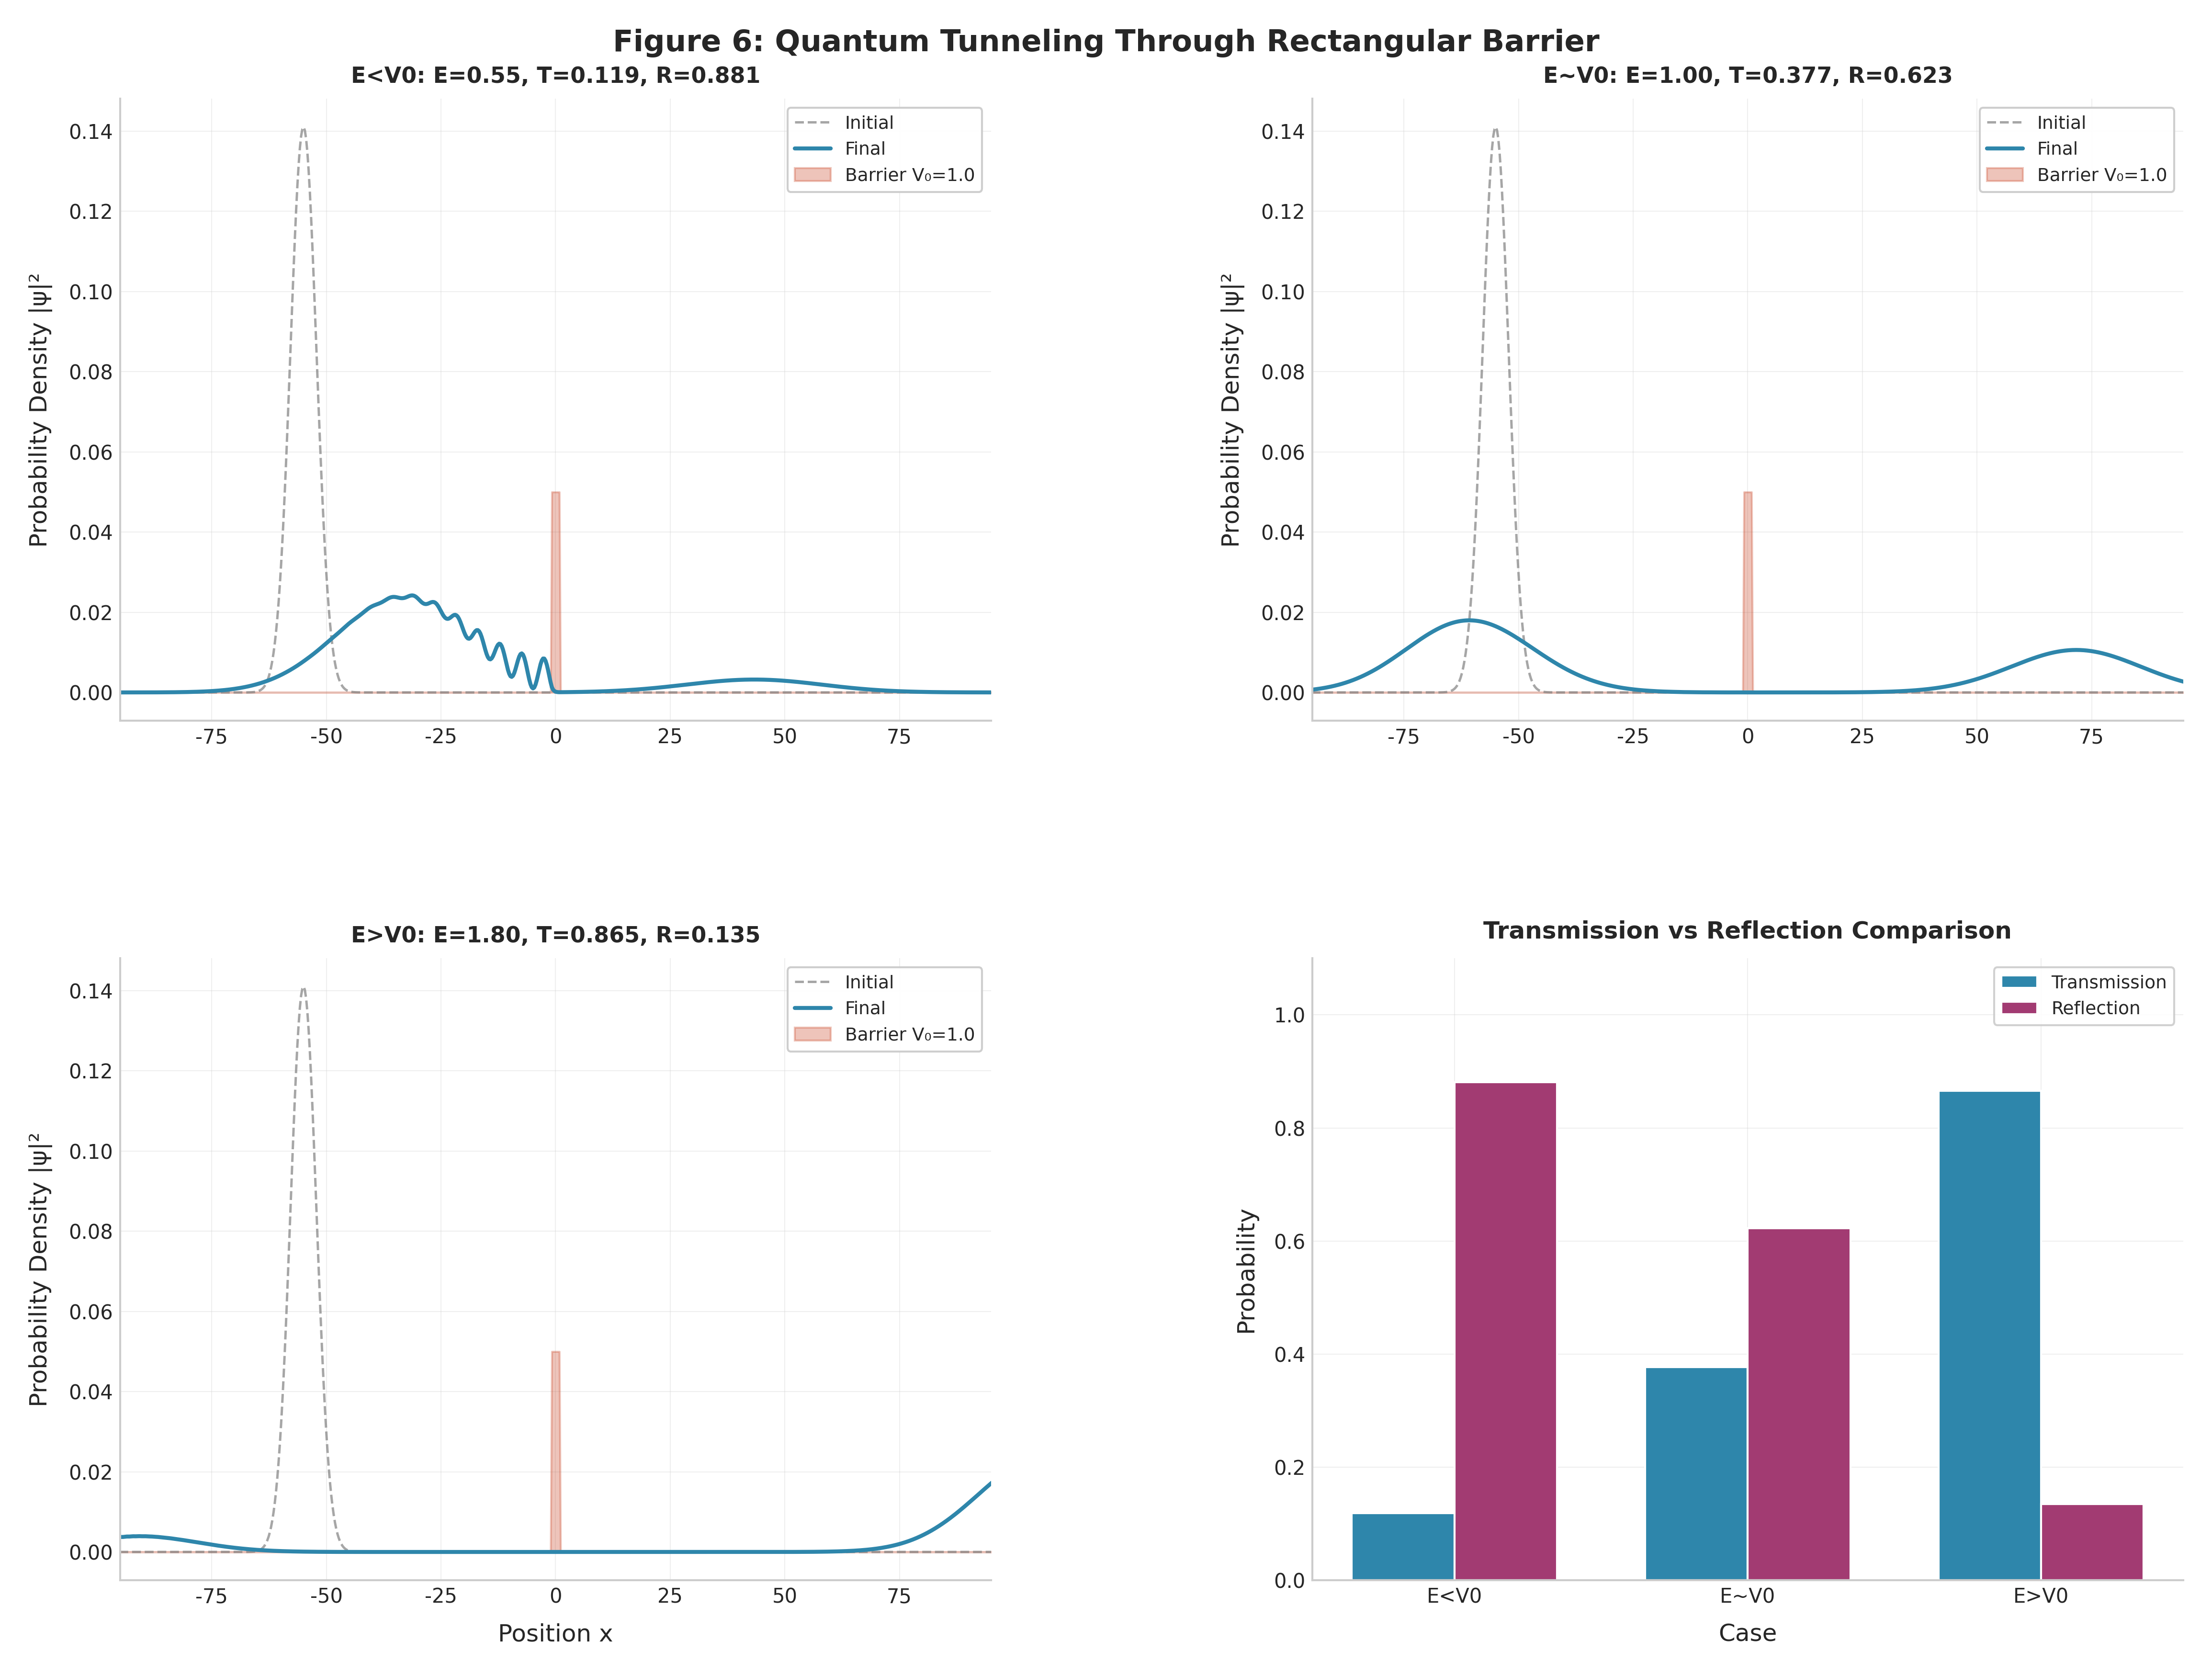
\includegraphics[width=0.85\textwidth]{figure6_tunneling_simulation.png}
\caption{量子隧穿模拟：三种能量情形（$E<V_0$、$E\approx V_0$、$E>V_0$）下波包与矩形势垒的相互作用，右下为透射/反射概率柱状图对比}
\label{fig:1d_tunneling}
\end{figure}

图~\ref{fig:1d_tunneling_reim} 进一步展示了 $E<V_0$ 情形下势垒附近的实部和虚部分布。从中可以清楚地观察到：
\begin{itemize}
    \item 势垒\textbf{左侧}（入射+反射区）：$\mathrm{Re}[\psi]$ 和 $\mathrm{Im}[\psi]$ 呈现明显的驻波干涉图样——入射波与反射波叠加形成的空间振荡，二者相位差约 $\pi/2$。
    \item 势垒\textbf{内部}：波函数指数衰减（经典禁区）。
    \item 势垒\textbf{右侧}（透射区）：$\mathrm{Re}[\psi]$ 和 $\mathrm{Im}[\psi]$ 平缓且幅值较小，对应隧穿透射波。
\end{itemize}
这些干涉图样在 $|\psi|^2$ 图（图~\ref{fig:1d_tunneling}）中仅表现为平滑的指数衰减包络，\textbf{完全丢失了波函数的振荡结构和相位信息}。这正是三值分析方法的价值所在。

\begin{figure}[H]
\centering
\includegraphics[width=0.85\textwidth]{figure6b_tunneling_re_im.png}
\caption{隧穿波函数的实部与虚部（$E<V_0$ 情形）：势垒左侧的振荡展示入射波与反射波的干涉图样（$|\psi|^2$ 中不可见），右侧平缓衰减对应隧穿透射波}
\label{fig:1d_tunneling_reim}
\end{figure}

\subsection{多格式综合对比：谐振子势中的三值视图}

图~\ref{fig:1d_method_cmp} 展示了在弱谐振子势（$\omega=0.1$）中，五种格式从相同初始条件出发经过 $t=1.5$ 演化后的结果对比。同样采用三面板布局（$|\psi|^2$、$\mathrm{Re}[\psi]$、$\mathrm{Im}[\psi]$），可以直观比较各格式在势场约束下的表现差异。

\begin{figure}[H]
\centering
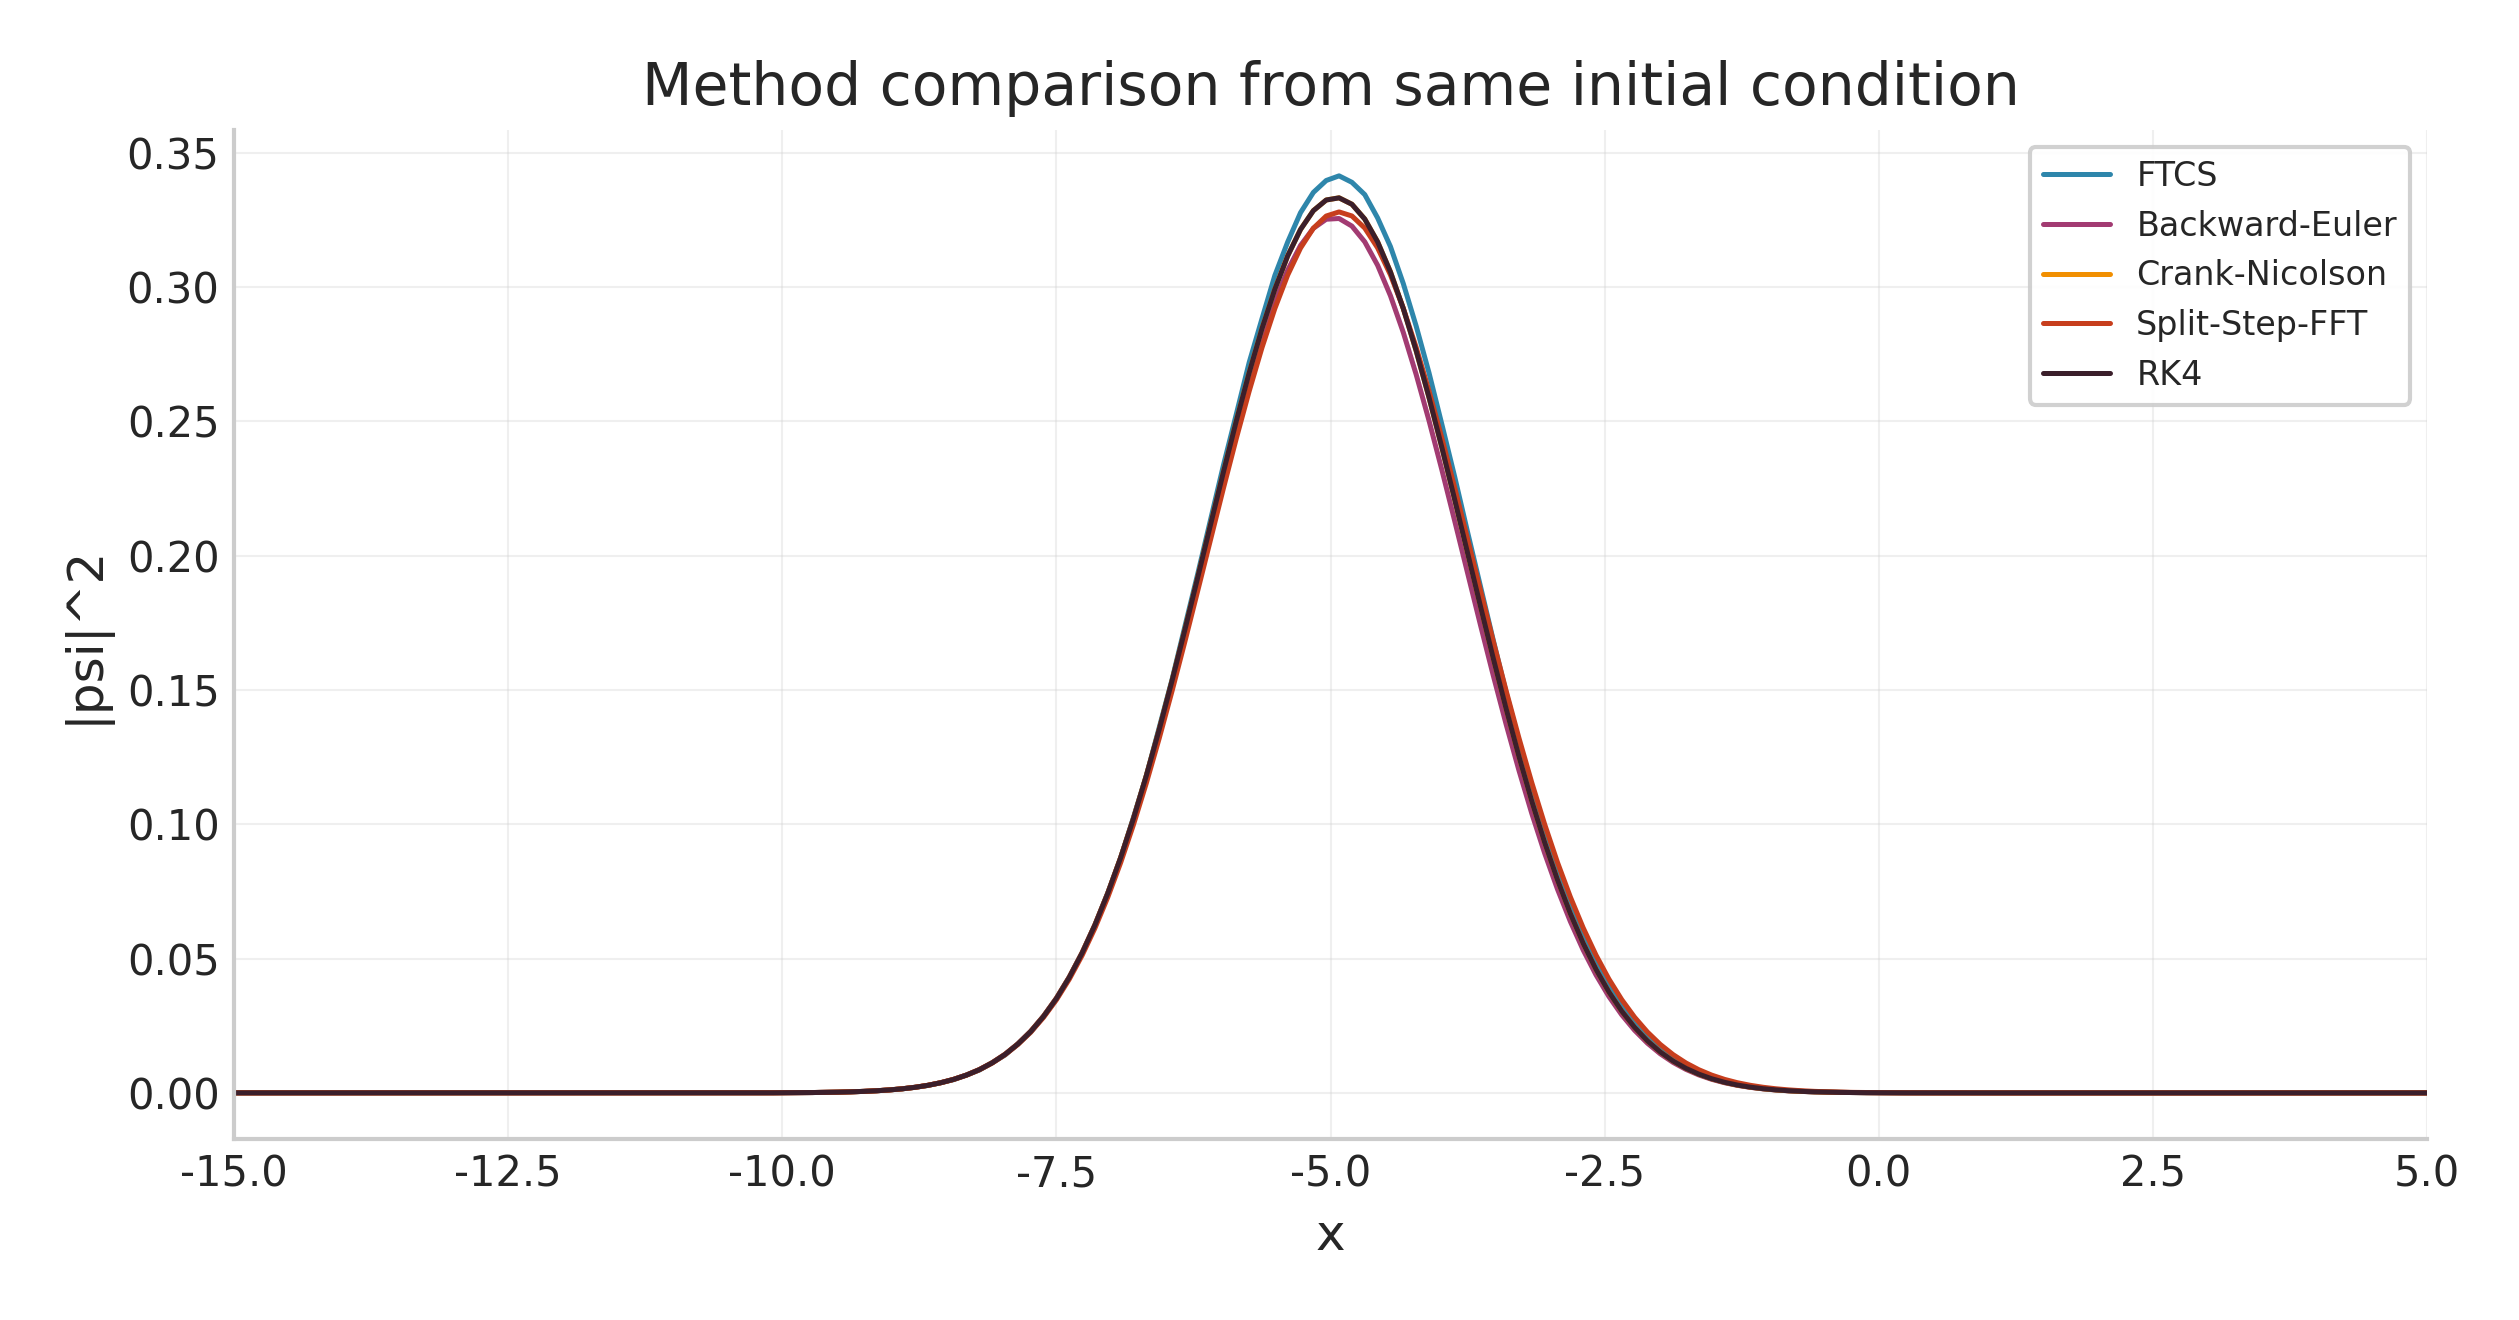
\includegraphics[width=0.85\textwidth]{method_comparison.png}
\caption{五种一维格式在弱谐振子势（$\omega=0.1$）中的演化对比——\textbf{三值视图}：$|\psi|^2$（左）、$\mathrm{Re}[\psi]$（中）、$\mathrm{Im}[\psi]$（右）}
\label{fig:1d_method_cmp}
\end{figure}

\subsection{双势垒共振隧穿（RTD）}

作为单势垒隧穿的推广，本文还模拟了双势垒共振隧穿二极管（Resonant Tunneling Diode, RTD）结构：两个相同的矩形势垒（$V_0=1.0$）位于 $x \in [-3.0, -1.5]$ 和 $x \in [1.5, 3.0]$，中间形成宽度为 $3.0$ 的量子阱。使用 Crank--Nicolson 格式模拟了三种能量情形。

\begin{figure}[H]
\centering
\includegraphics[width=0.85\textwidth]{figure_rtd_double_barrier.png}
\caption{双势垒共振隧穿（RTD）模拟：三种能量情形（非共振 $E<V_0$、近共振 $E\approx V_0$、超势垒 $E>V_0$）下的概率密度分布及透射/反射对比（Crank--Nicolson 格式）}
\label{fig:1d_rtd}
\end{figure}

与单势垒不同，双势垒结构中的量子阱支持准束缚态（quasi-bound states）。当入射能量与阱中准束缚能级匹配时，发生\textbf{共振隧穿}——即使 $E < V_0$（经典禁区），透射率 $T$ 也可接近 $1$。这是因为波函数在阱内被多次反射增强，形成了类似光学法布里-珀罗腔的共振透射机制。

图~\ref{fig:1d_rtd_reim} 给出了近共振情形下双势垒区域的实部和虚部分布。在量子阱内部（$x \in [-1.5, 1.5]$），波函数的实部和虚部呈现\textbf{强烈的驻波振荡}，幅值远大于外部区域——这正是准束缚态的典型特征。这种阱内的概率增强在 $|\psi|^2$ 图中也能观察到，但 Re/Im 视图额外揭示了振荡的相位结构。

\begin{figure}[H]
\centering
\includegraphics[width=0.85\textwidth]{figure_rtd_re_im.png}
\caption{双势垒近共振隧穿的实部与虚部（$E\approx V_0$，Crank--Nicolson）：阱内（$x\in[-1.5,1.5]$）呈现强烈的驻波振荡，展示准束缚态特征}
\label{fig:1d_rtd_reim}
\end{figure}

%==============================================================================
\section{二维数值实验结果}
%==============================================================================

\subsection{二维自由传播}

图~\ref{fig:2d_free} 展示了二维自由高斯波包在 $t=0$、$t=1.0$ 和 $t=2.0$ 三个时刻的 $|\psi|^2$ 密度分布热图，以及质量守恒曲线。Split-Step FFT 方法在二维自由传播中保持了极高的质量守恒精度（误差 $< 10^{-4}$）。

\begin{figure}[H]
\centering
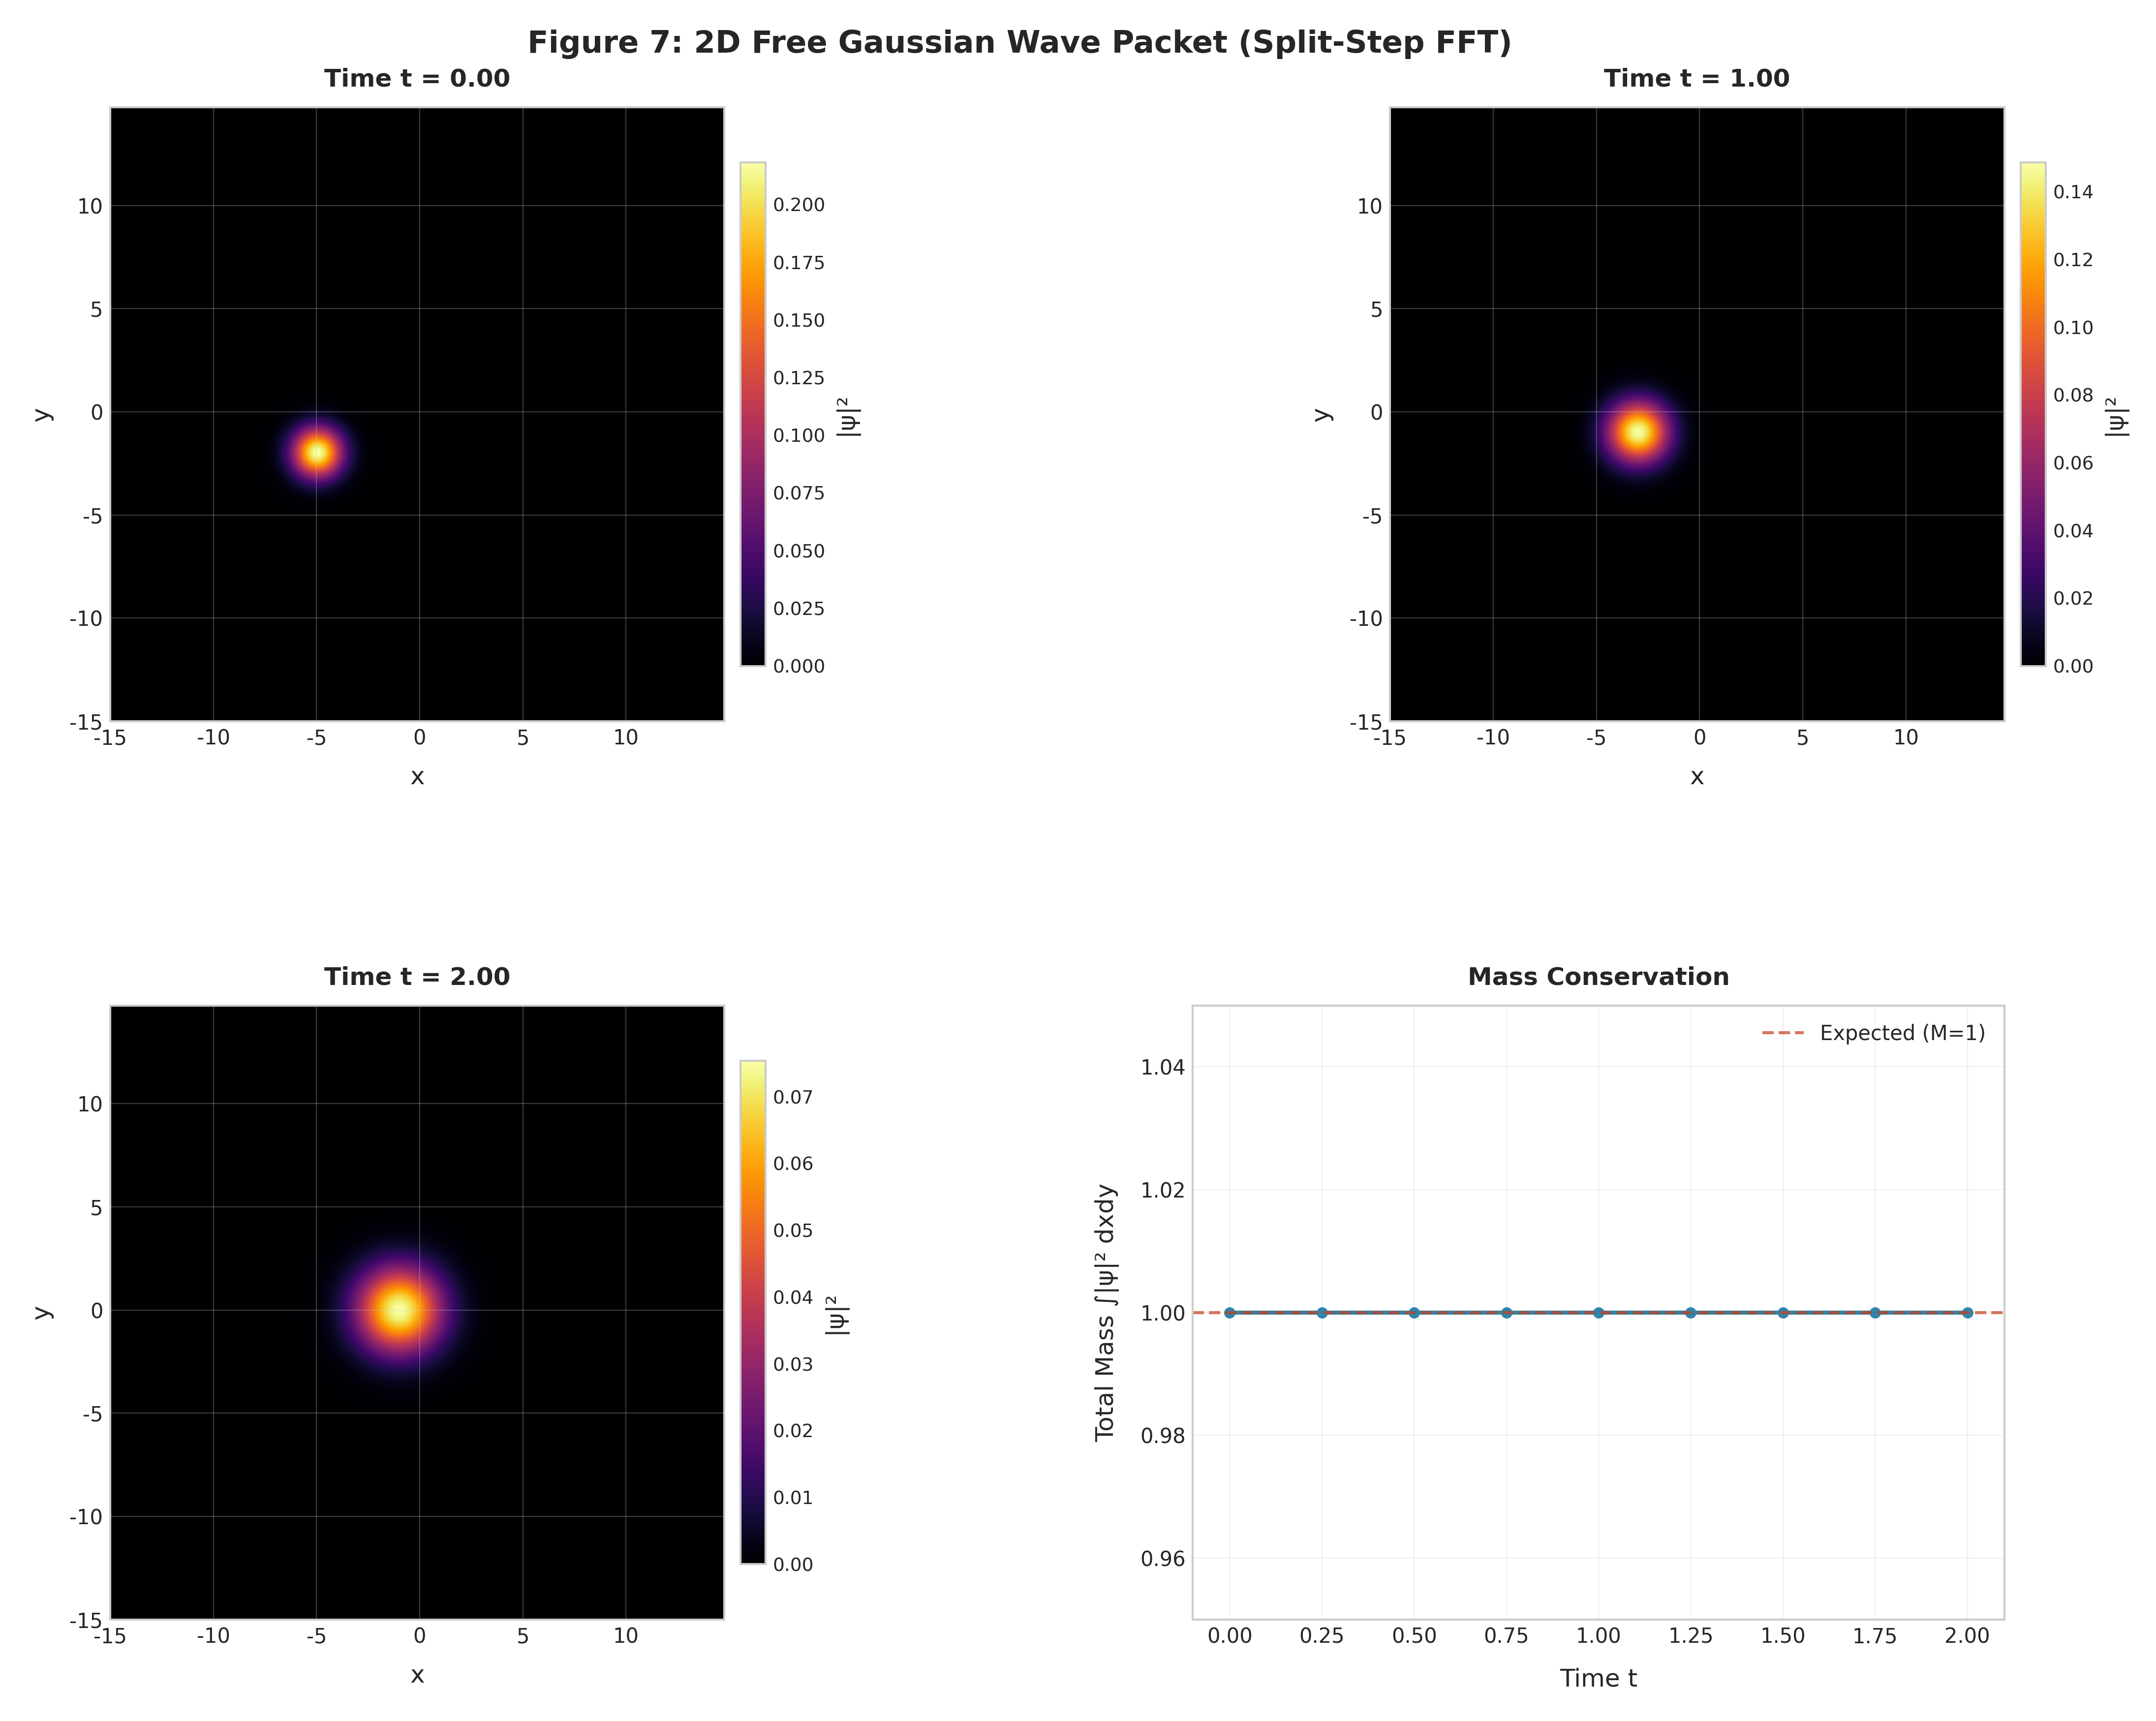
\includegraphics[width=0.85\textwidth]{figure7_2d_free_propagation.png}
\caption{二维自由高斯波包传播（Split-Step FFT）：三个时刻（$t=0, 1.0, 2.0$）的 $|\psi|^2$ 密度热图及质量守恒曲线}
\label{fig:2d_free}
\end{figure}

图~\ref{fig:2d_free_phase} 补充展示了相同三个时刻的相位角 $\arg\psi(x,y)$ 分布。与密度热图仅显示波包位置不同，相位角热图直观地揭示了波前（wavefront）的结构：相位梯度 $\nabla\arg\psi$ 指向局部传播方向，等相位线的间距反映局部波长。

\begin{figure}[H]
\centering
\includegraphics[width=0.95\textwidth]{figure7b_2d_phase_angle.png}
\caption{二维自由传播的相位角 $\arg\psi$ 分布（三个时刻）：波前传播可视化，等相位线的间距和运动反映波包的传播方向和局部波长}
\label{fig:2d_free_phase}
\end{figure}

\subsection{圆形障碍物散射}

图~\ref{fig:2d_scatter} 展示了高斯波包（$k_{x0}=3.0$）入射圆形障碍物（半径 $R=1.5$，势高 $V_0=20.0$）的散射过程。三个时刻分别对应：初始状态、接近障碍物、散射后的波包形态。右下子图展示了散射角的角分布直方图，呈现明显的前向散射为主、伴有后向散射的特征。该实验使用了复值吸收边界势以消除周期性回绕。

\begin{figure}[H]
\centering
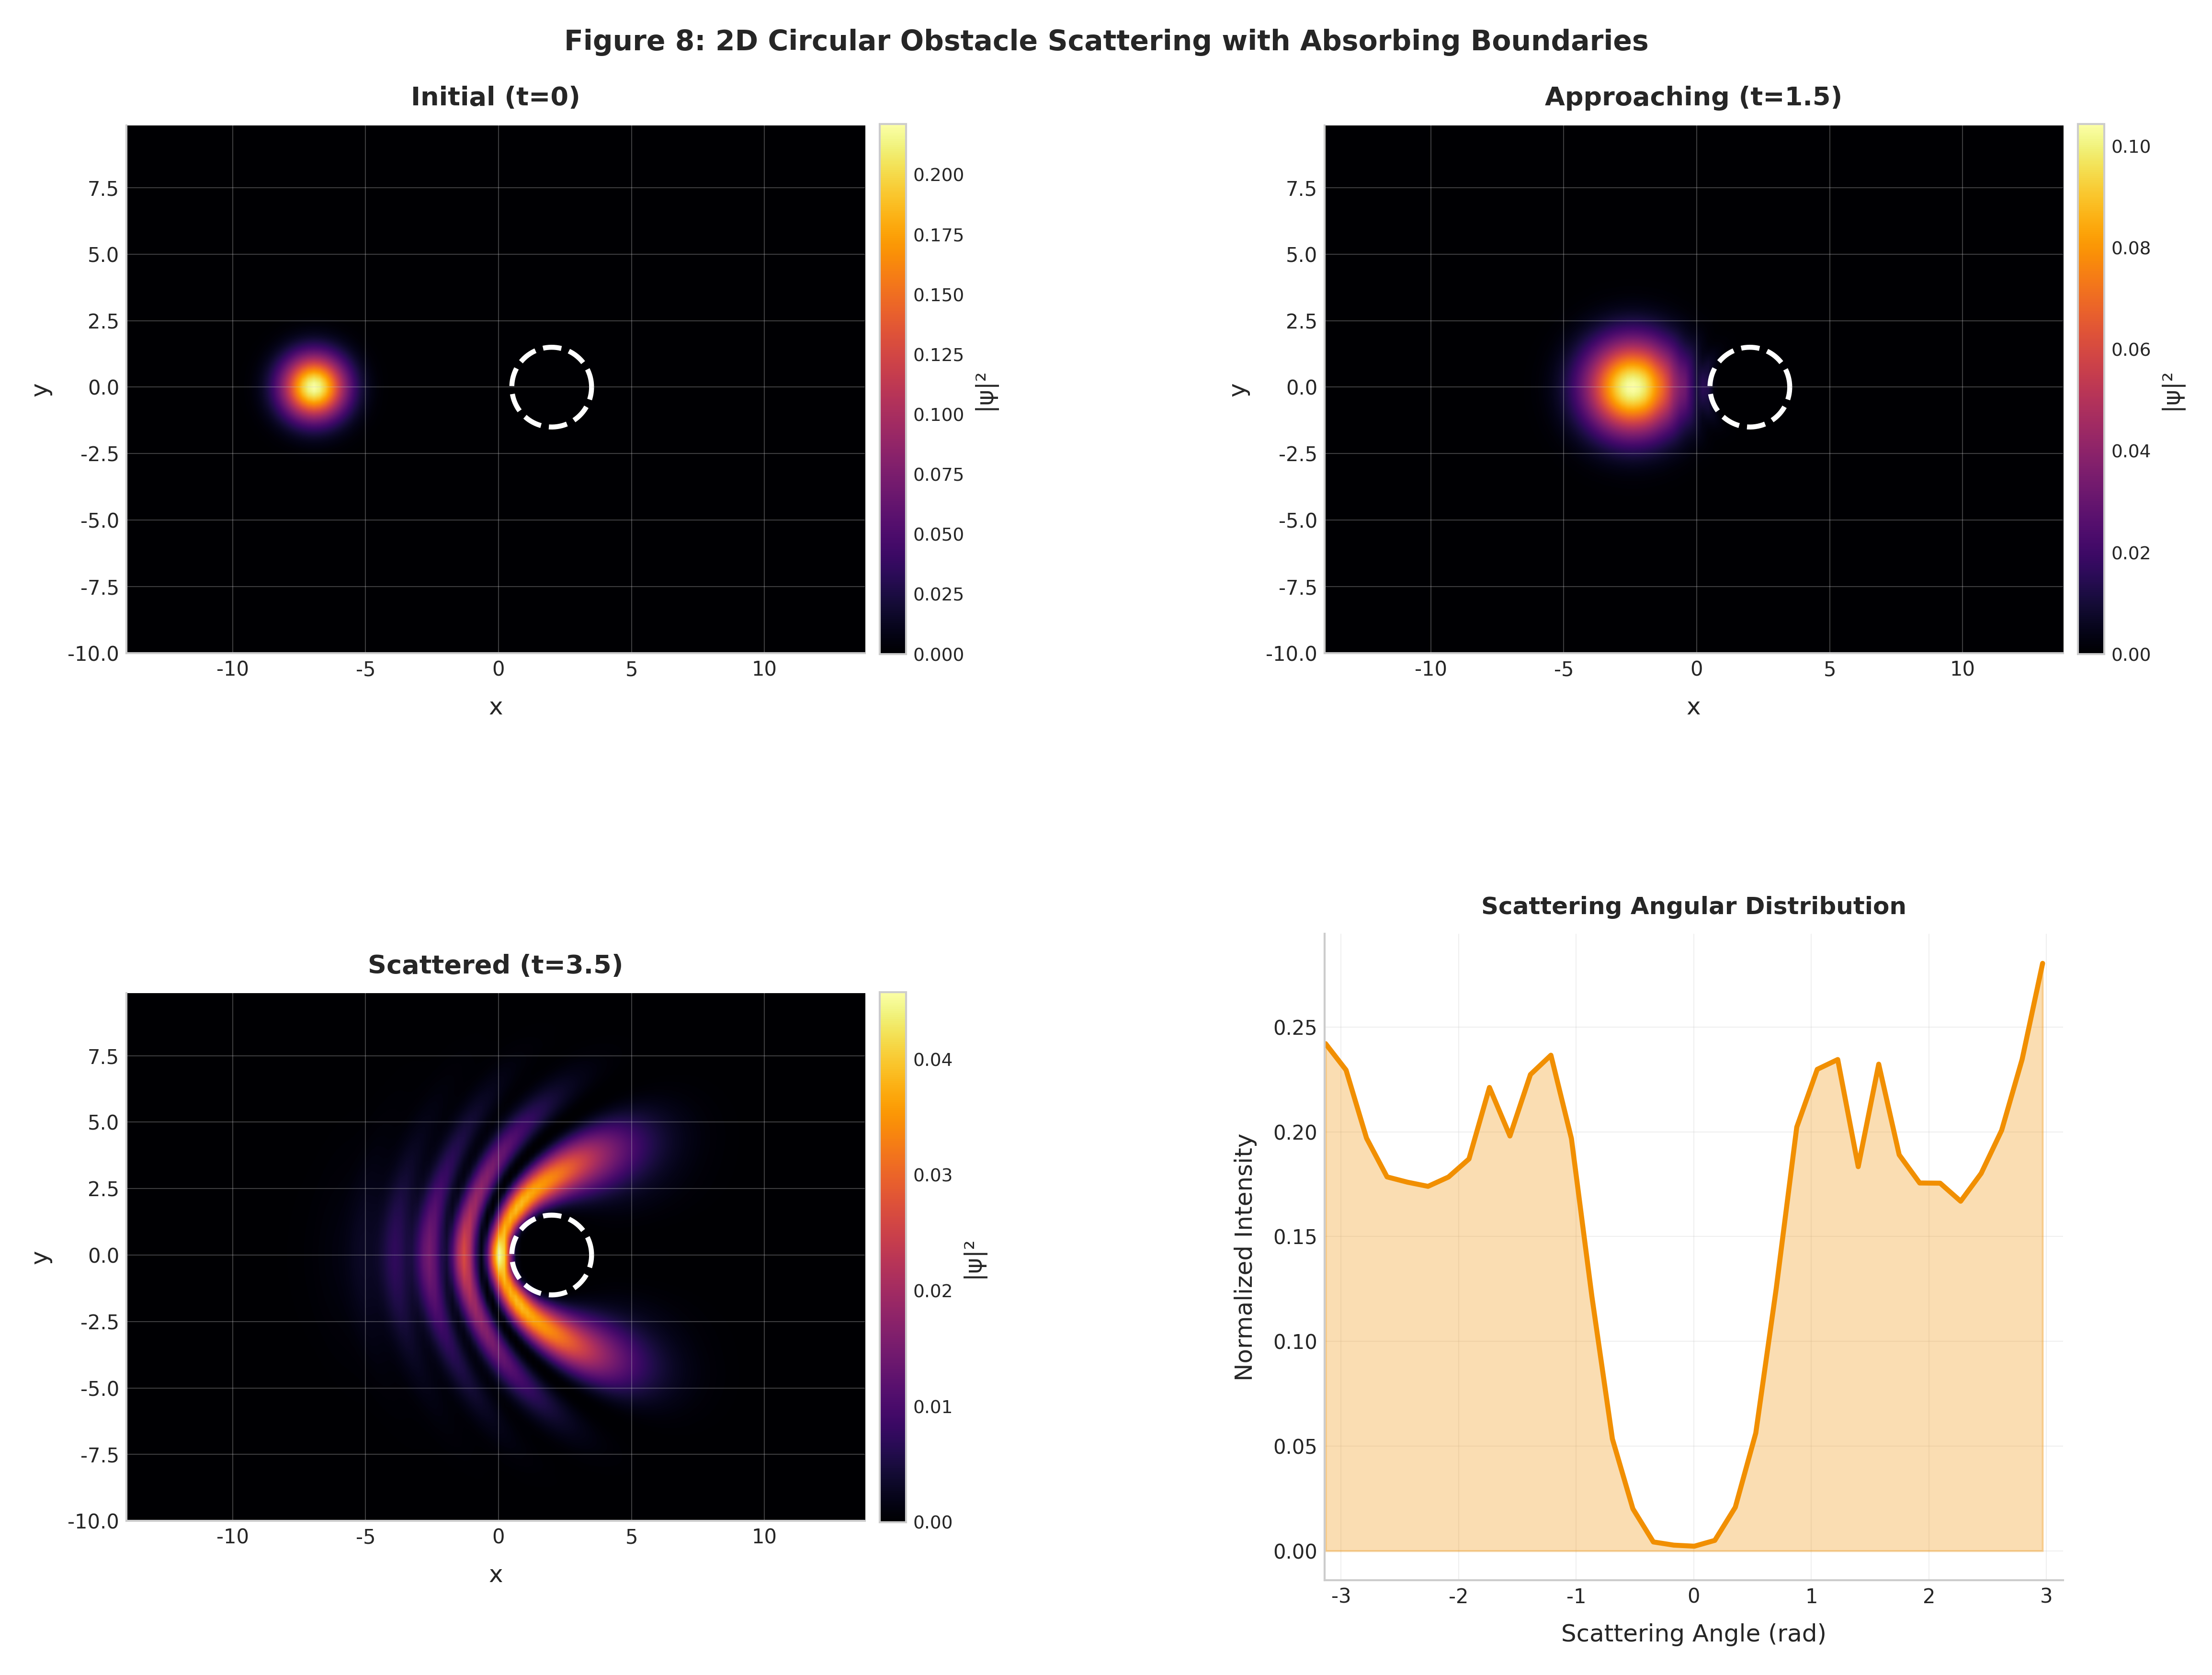
\includegraphics[width=0.85\textwidth]{figure8_2d_circular_obstacle_absorbing.png}
\caption{二维圆形障碍物散射：初始、接近和散射后三个时刻的 $|\psi|^2$ 密度热图（白色虚线圆标记障碍物边界），右下为散射角分布}
\label{fig:2d_scatter}
\end{figure}

\subsection{抛物型波导约束传播}

图~\ref{fig:2d_waveguide} 对比了同一高斯波包在自由空间和抛物型波导（$V(x,y) = 0.4y^2$）中的传播行为。上方为 $t=t_{\text{final}}$ 时的 $|\psi|^2$ 密度热图，下方为横向（$y$ 方向）边际概率分布 $\int |\psi|^2 dx$。

\begin{figure}[H]
\centering
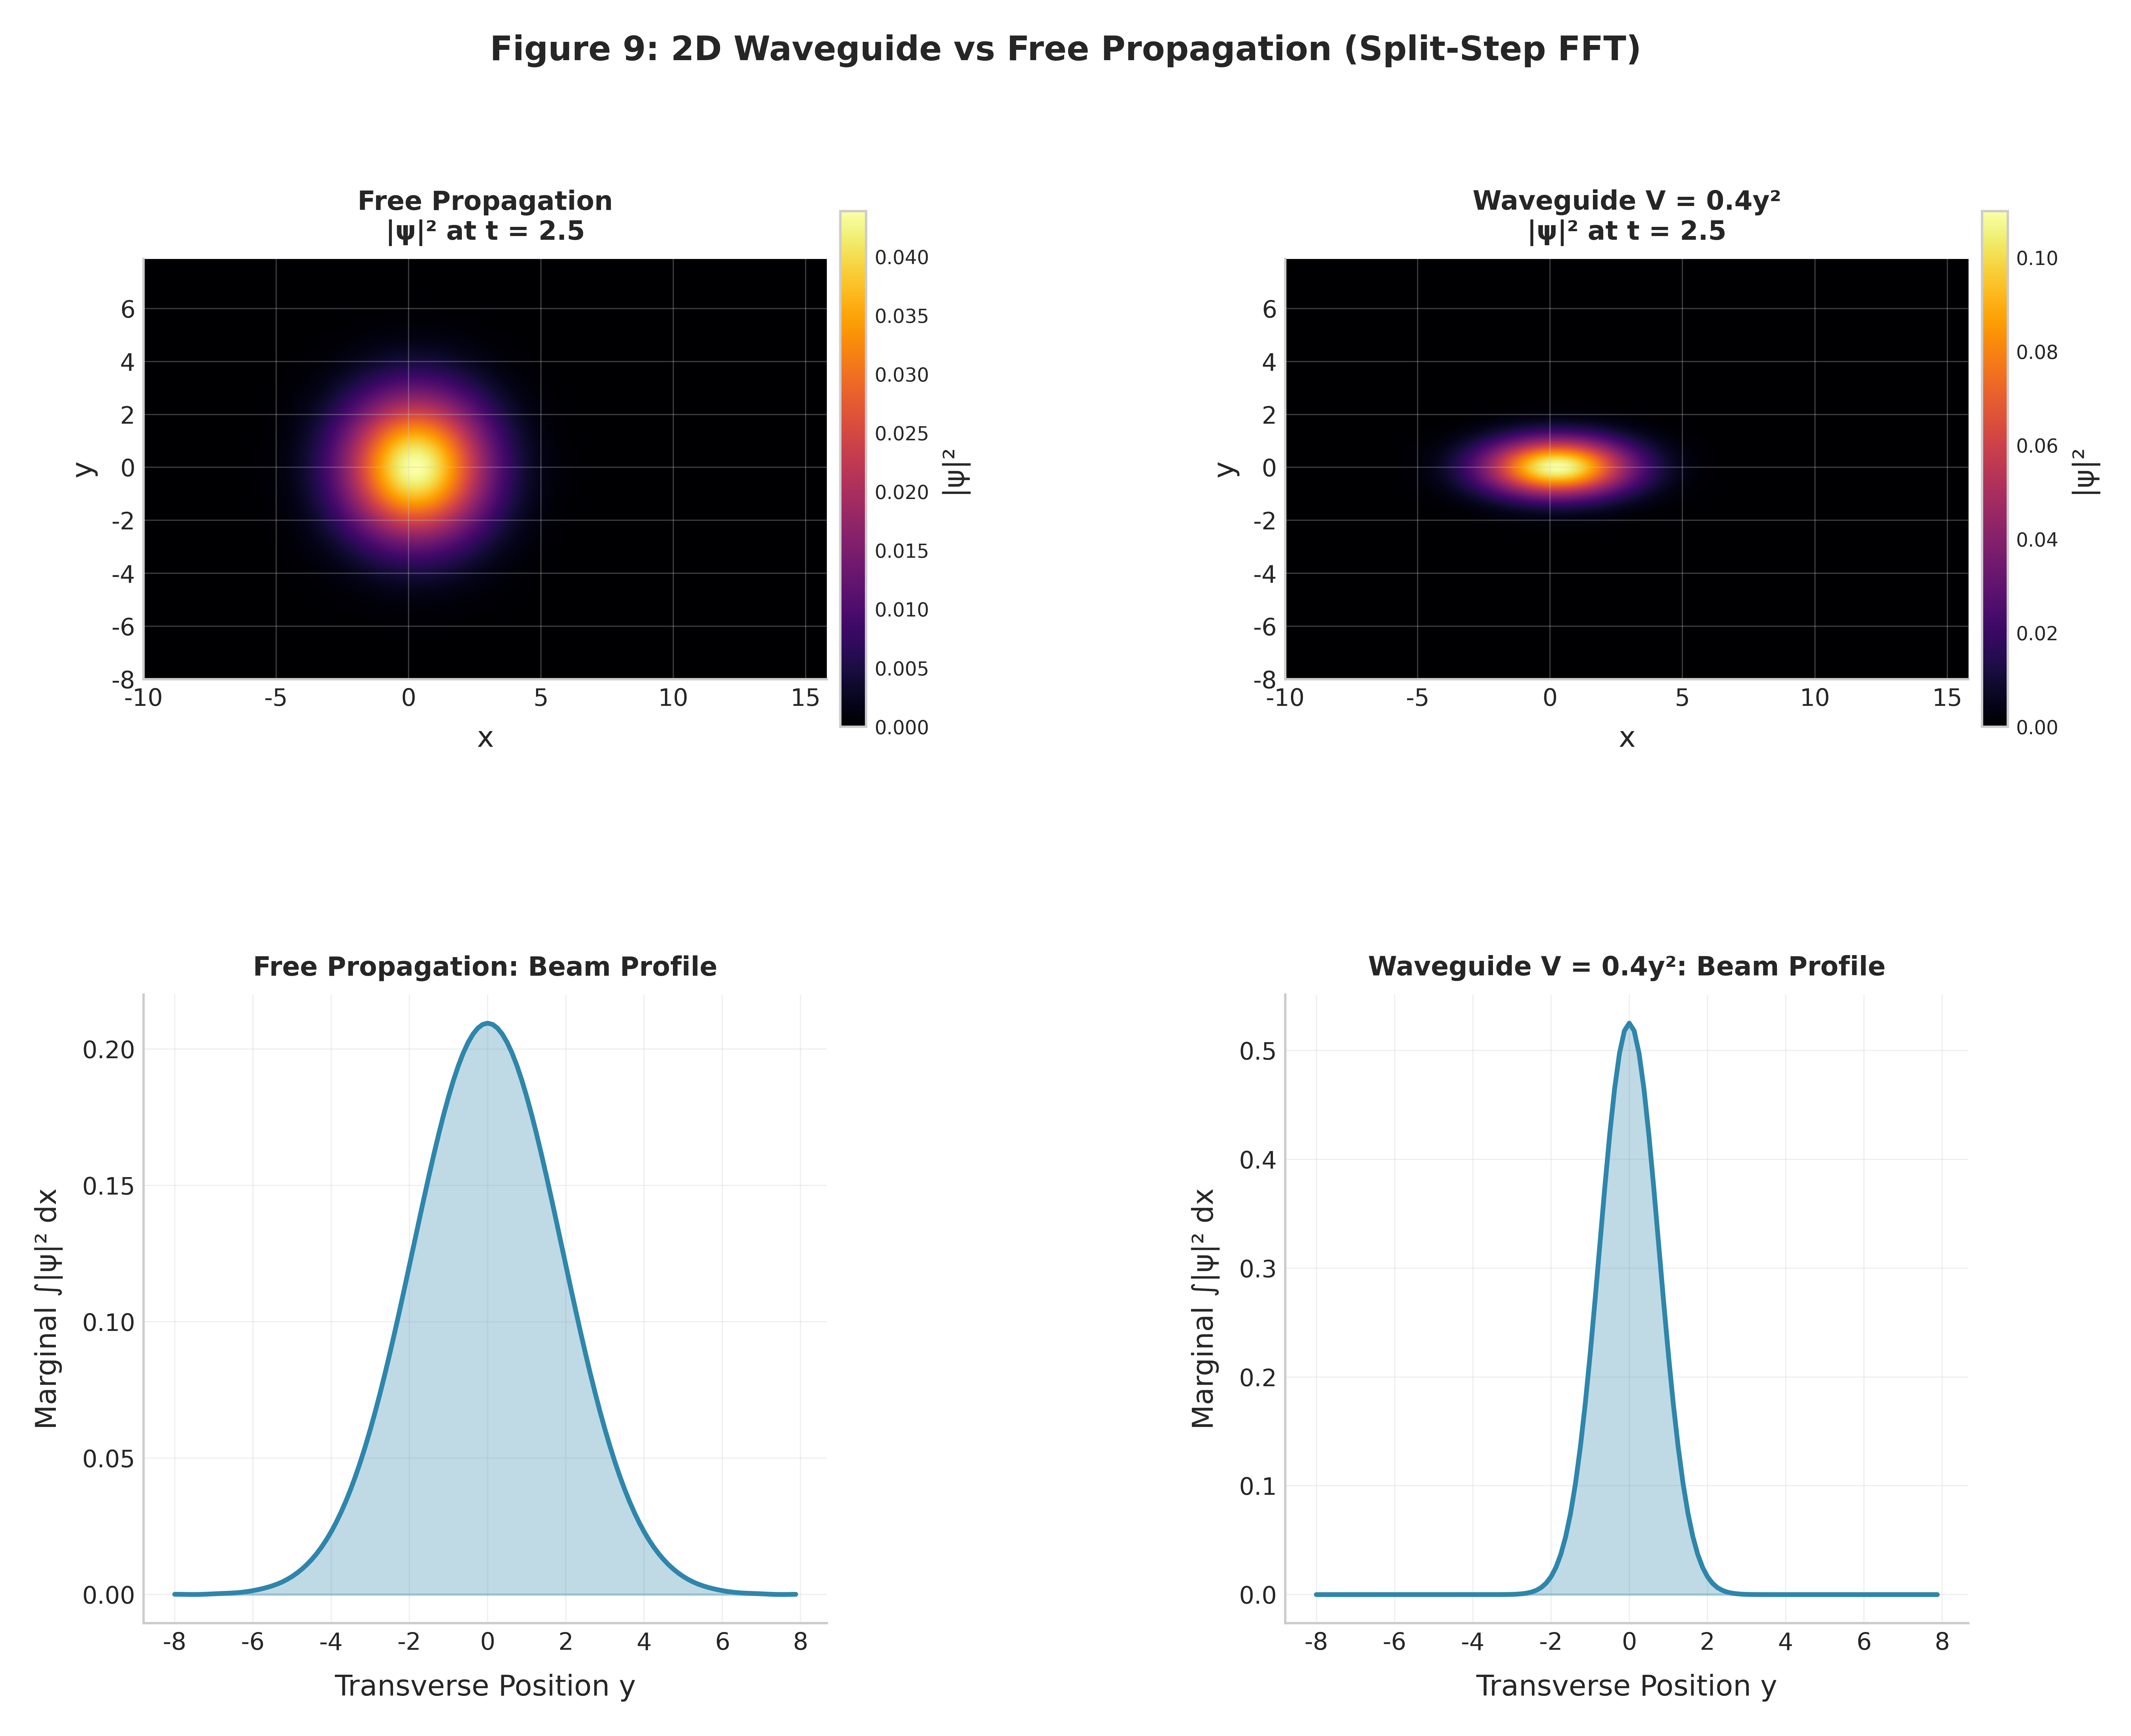
\includegraphics[width=0.80\textwidth]{figure9_2d_waveguide.png}
\caption{二维波导约束传播：自由传播（左）与波导约束（右，$V=0.4y^2$）的 $|\psi|^2$ 热图对比（上排）及横向束流剖面（下排）}
\label{fig:2d_waveguide}
\end{figure}

从图中可以清楚看到：自由传播中波包在 $y$ 方向迅速扩散（束流变宽），而在波导中横向约束使波包保持窄束形态沿 $x$ 方向定向传播。下方边际分布定量显示了波导的约束效果——波导中的束流宽度显著小于自由传播。

%==============================================================================
\section{数值分析}
%==============================================================================

\subsection{全方法综合对比与实/虚部误差分解}\label{sec:all_methods_cmp}

图~\ref{fig:all_methods} 将五种一维数值格式在同一自由高斯波包基准上进行了全面的"体检"。该六面板图包含：

\begin{figure}[H]
\centering
\includegraphics[width=0.95\textwidth]{figure_all_methods_comparison.png}
\caption{全方法综合对比：六面板——(1) $|\psi|^2$ 叠合曲线；(2) $L_2$ 误差柱状图（对数坐标）；(3) 质量误差柱状图；（4）运行时间对比；(5) 效率（误差/时间）；(6) 最佳格式与精确解的 $\mathrm{Re}[\psi]/\mathrm{Im}[\psi]$ 对比}
\label{fig:all_methods}
\end{figure}

\begin{itemize}
    \item \textbf{面板 1}（$|\psi|^2$ 叠合）：直观展示各格式的概率密度吻合程度。
    \item \textbf{面板 2}（$L_2$ 误差，对数坐标）：量化各格式的整体误差水平。
    \item \textbf{面板 3}（质量误差）：检验酉性——CN 和 SSF 的质量误差应在机器精度级别（$<10^{-14}$），BE 有显著耗散。
    \item \textbf{面板 4}（运行时间）：计算效率对比。
    \item \textbf{面板 5}（效率指标 = 误差/时间）：综合考量精度和速度。
    \item \textbf{面板 6}（$\mathrm{Re}[\psi]/\mathrm{Im}[\psi]$ 对比）：最佳非 FTCS 格式与精确解的实部和虚部逐点对比。
\end{itemize}

此外，输出数据表格中包含了各格式的\textbf{实/虚部 $L_2$ 误差分解}：
\begin{equation}
    L_2^{\mathrm{Re}} = \|\mathrm{Re}[\psi_{\text{num}} - \psi_{\text{ref}}]\|_{L^2}, \quad
    L_2^{\mathrm{Im}} = \|\mathrm{Im}[\psi_{\text{num}} - \psi_{\text{ref}}]\|_{L^2}.
\end{equation}
如果一个格式的 $L_2^{\mathrm{Re}} \gg L_2^{\mathrm{Im}}$（或反之），说明误差主要集中在某一侧，表明存在\textbf{系统性相位漂移}而非单纯的均匀振幅衰减。非酉格式（如 Backward Euler）通常表现出这种不平衡性，而酉格式（CN、SSF）在实部和虚部上的误差更为均衡。

\subsection{一维质量守恒（酉性）分析}

图~\ref{fig:conservation} 展示了 FTCS、Crank--Nicolson 和 Split-Step FFT 三种格式的质量误差 $|M(t)-M(0)|$ 随时间的变化（半对数坐标）。

\begin{figure}[H]
\centering
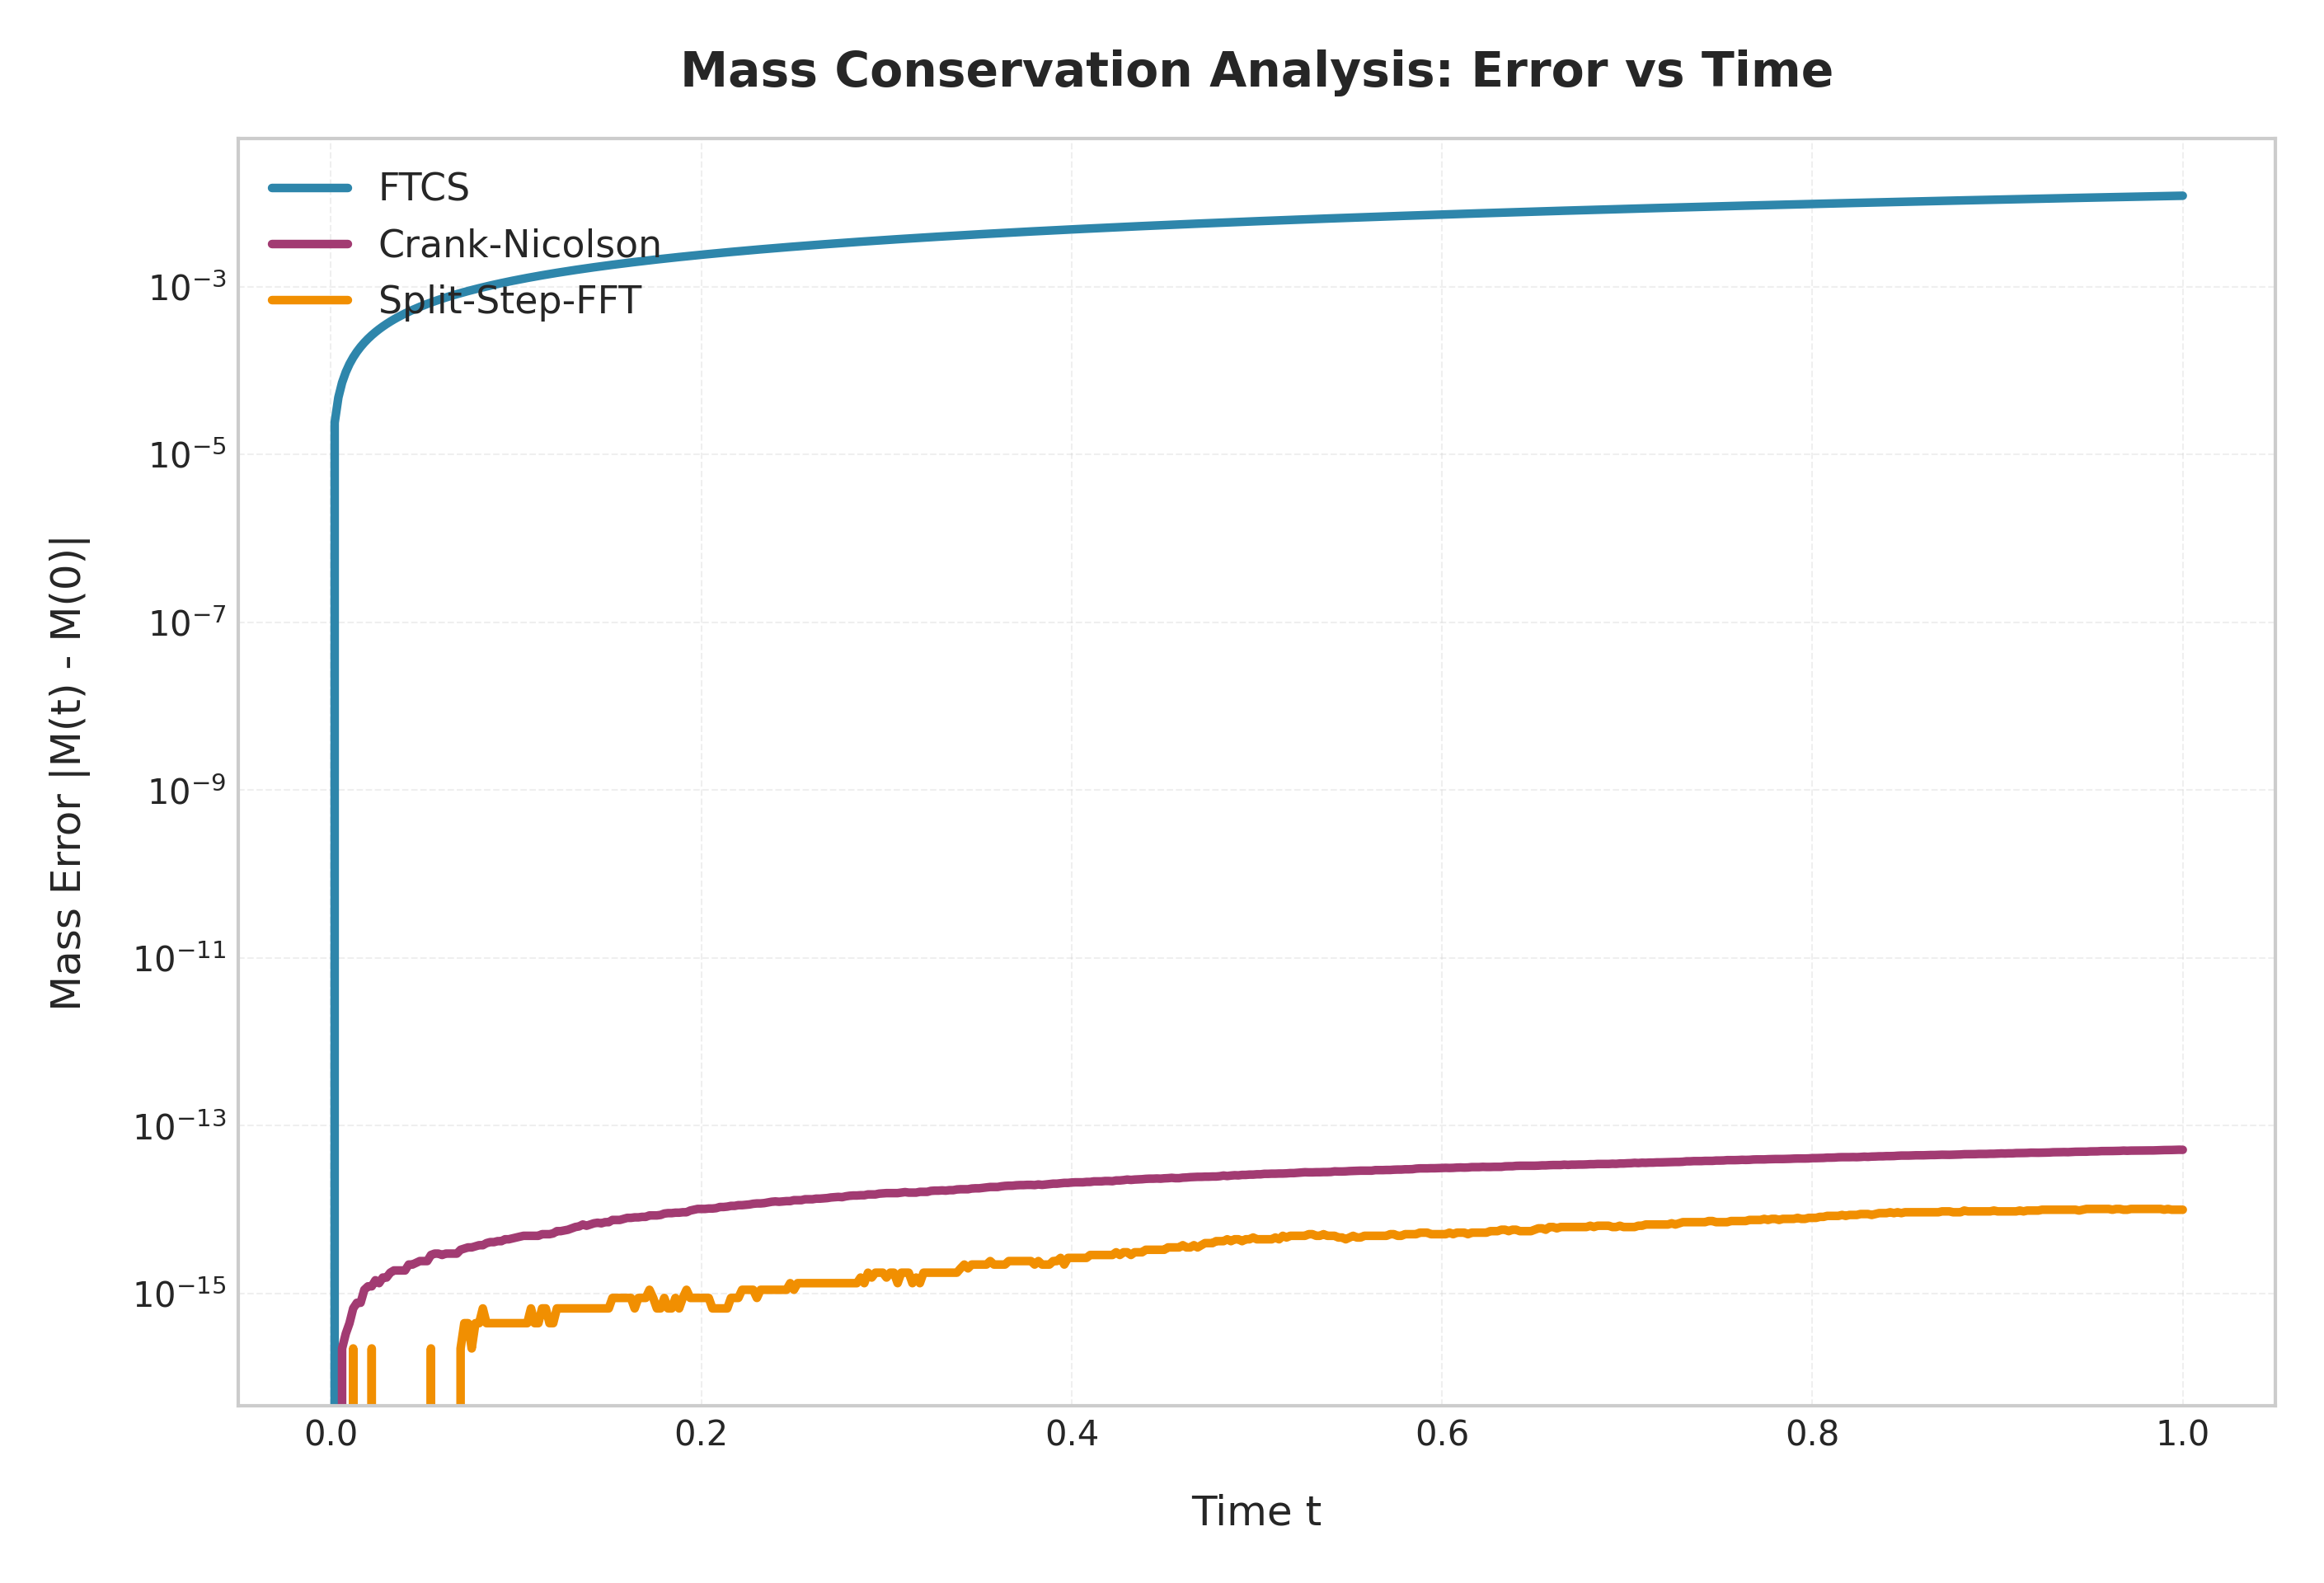
\includegraphics[width=0.70\textwidth]{figure_conservation_analysis.png}
\caption{一维质量守恒分析：三种格式的质量误差 $|M(t)-M(0)|$ 随时间的变化（半对数坐标）——FTCS 迅速发散，CN 和 SSF 保持在机器精度附近}
\label{fig:conservation}
\end{figure}

结果表明：
\begin{itemize}
    \item \textbf{FTCS}：质量误差呈指数增长（不稳定格式的必然结果）。
    \item \textbf{Crank--Nicolson} 和 \textbf{Split-Step FFT}：整个模拟时间内质量误差保持在 $10^{-14}$ 量级（机器精度附近），充分体现了\textbf{酉格式}的守恒优势。
\end{itemize}

这一实验是对表~\ref{tab:methods} 中"酉性"列的直接数值验证。

\subsection{运行时间详细对比}

图~\ref{fig:runtime} 以表格形式展示了 FTCS、Crank--Nicolson 和 Split-Step FFT 在相同计算规模（$N=384$，500 步）下的详细运行数据，包括运行时间、初始质量、最终质量和质量误差。

\begin{figure}[H]
\centering
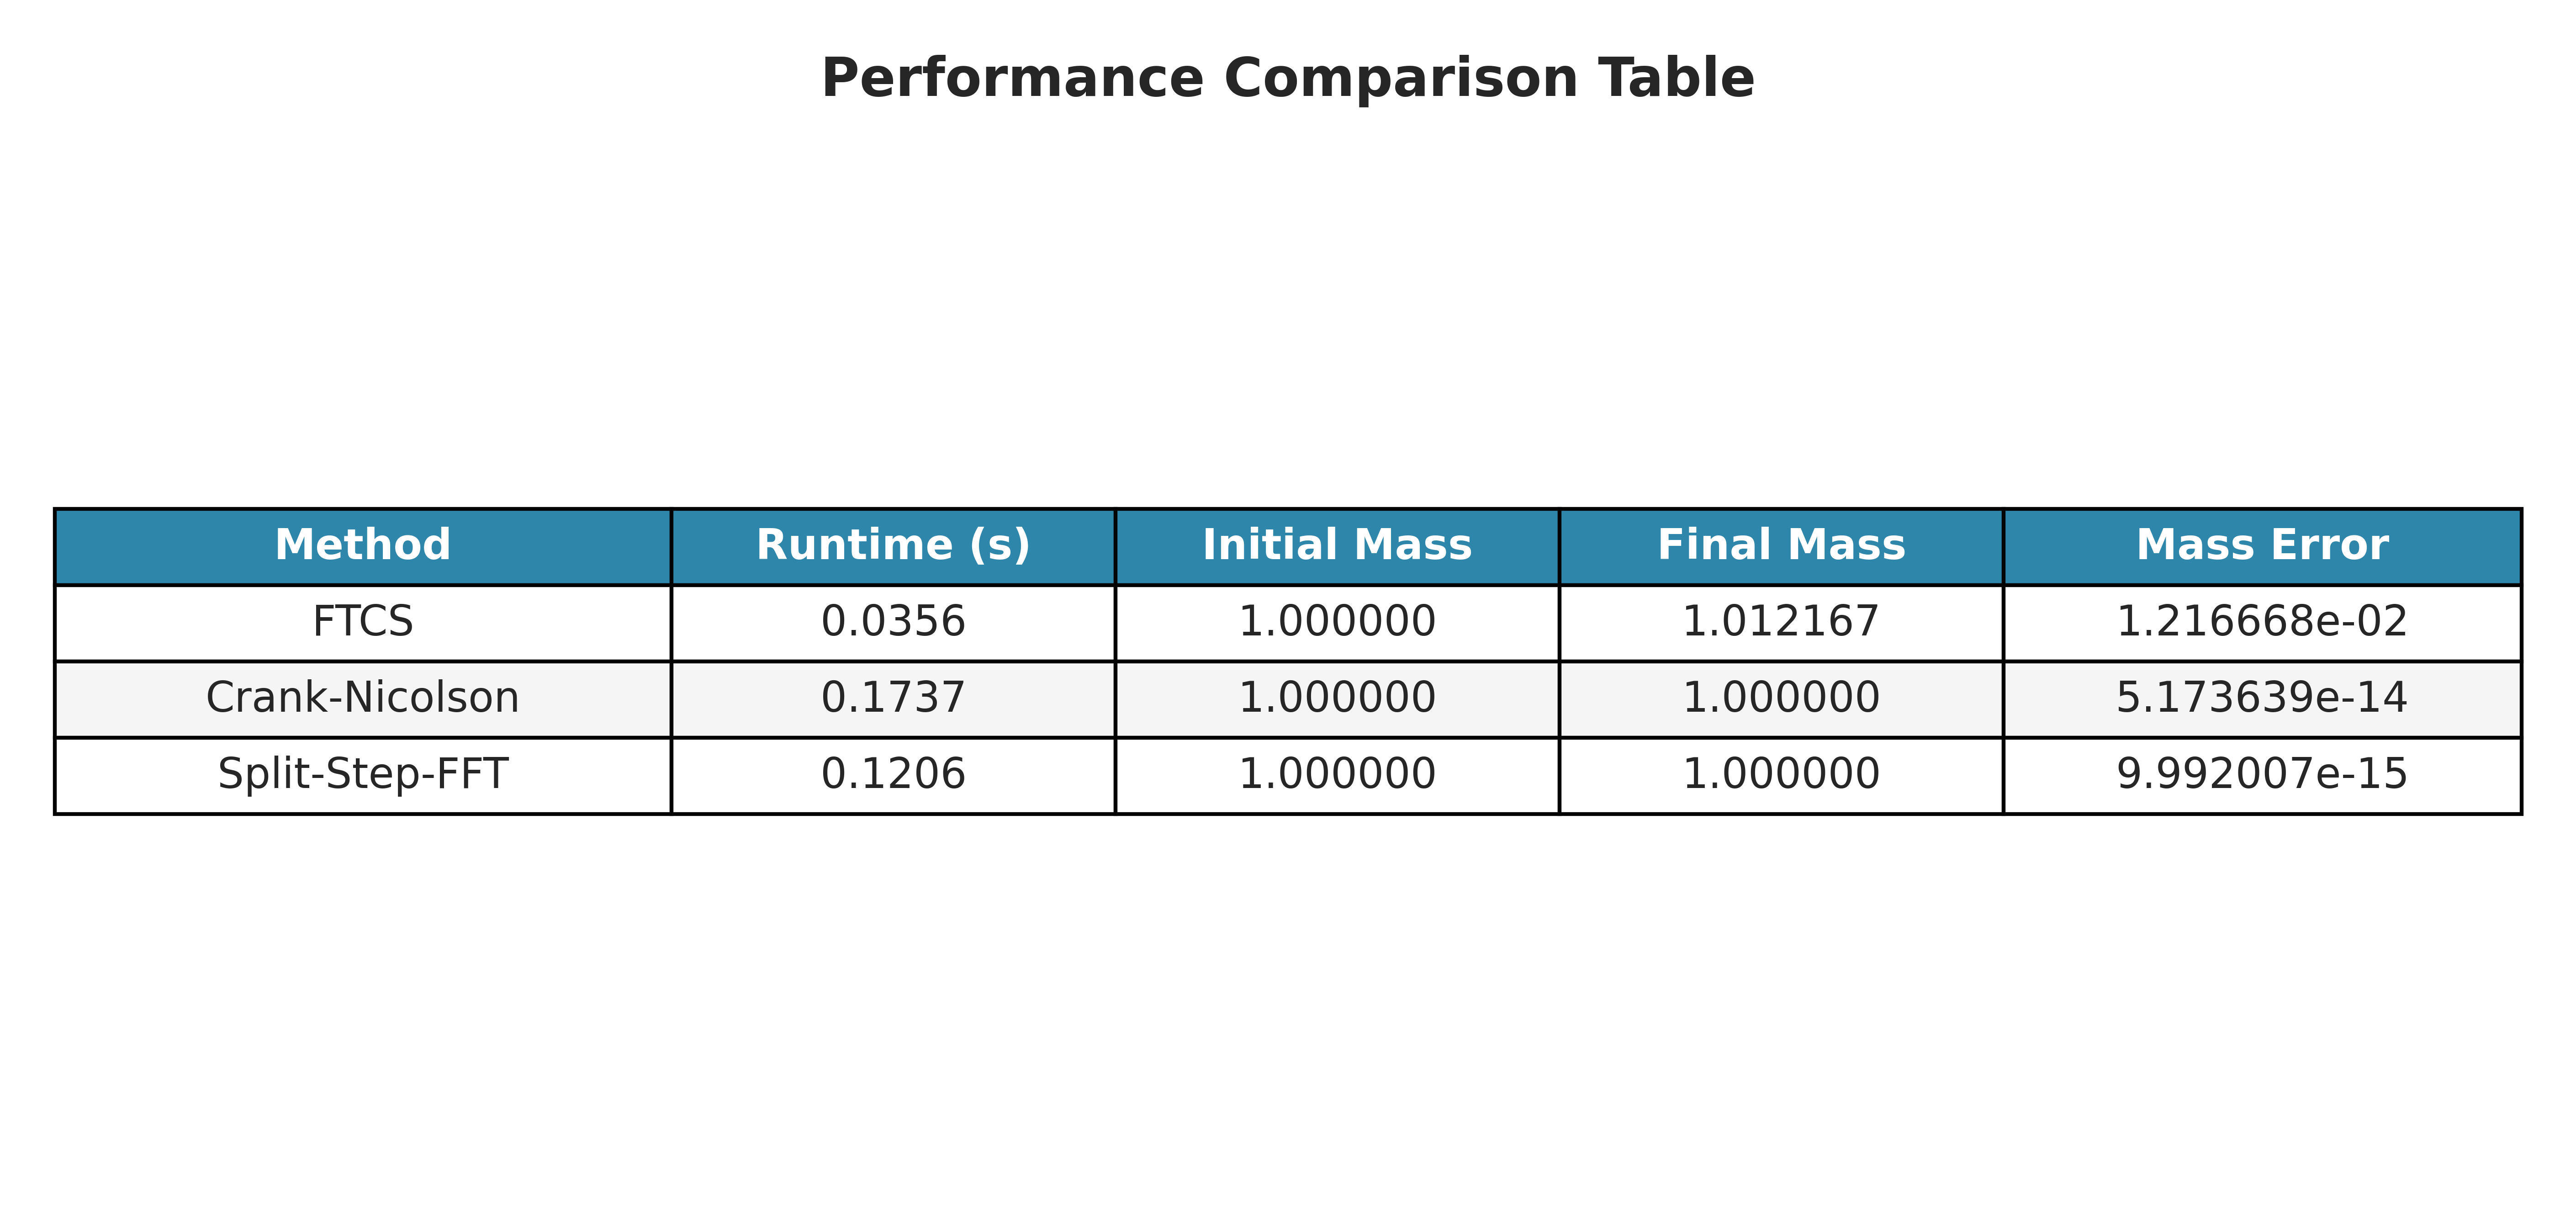
\includegraphics[width=0.80\textwidth]{figure_runtime_comparison.png}
\caption{一维格式运行时间及质量守恒详细对比表}
\label{fig:runtime}
\end{figure}

\subsection{二维 ADI vs Split-Step FFT 直接对比}

图~\ref{fig:2d_adi_ssf} 展示了二维 ADI 方法与 Split-Step FFT 方法在两个物理场景（自由传播、波导约束）下的头对头直接对比。每种场景包含三列：ADI 的 $|\psi|^2$、SSF 的 $|\psi|^2$、以及两者的逐点差值 $|\psi_{\text{ADI}} - \psi_{\text{SSF}}|$。

\begin{figure}[H]
\centering
\includegraphics[width=0.95\textwidth]{figure_2d_adi_vs_ssf.png}
\caption{二维 ADI vs Split-Step FFT 直接对比：两行分别为自由传播和波导约束场景；三列为 ADI $|\psi|^2$、SSF $|\psi|^2$、逐点差值 $|\Delta\psi|$（附 $L_2$ 差异值）}
\label{fig:2d_adi_ssf}
\end{figure}

对比结果表明：
\begin{itemize}
    \item 两种方法在自由传播和波导约束下的 $|\psi|^2$ 分布高度一致。
    \item 逐点差值 $|\Delta\psi|$ 主要集中在波包边缘（梯度大的区域），内部区域差异极小。
    \item $L_2$ 差异在 $10^{-4}$--$10^{-3}$ 量级，表明两种方法精度相当。
    \item ADI 通过每个方向的三对角求解实现无条件稳定（无需 FFT），适用于非周期边界条件；SSF 利用 FFT 达到谱精度并在周期边界条件下保持完美酉性。
\end{itemize}

\subsection{参数扫描实验}

\subsubsection{圆形障碍物半径扫描}

图~\ref{fig:circular_sweep} 展示了圆形障碍物半径 $R$ 从 $0.5$ 到 $2.5$ 变化时，透射质量和散射质量的变化趋势。随着障碍物半径增大，遮挡面积增加，透射质量单调递减，散射质量单调递增，符合物理直觉。

\begin{figure}[H]
\centering
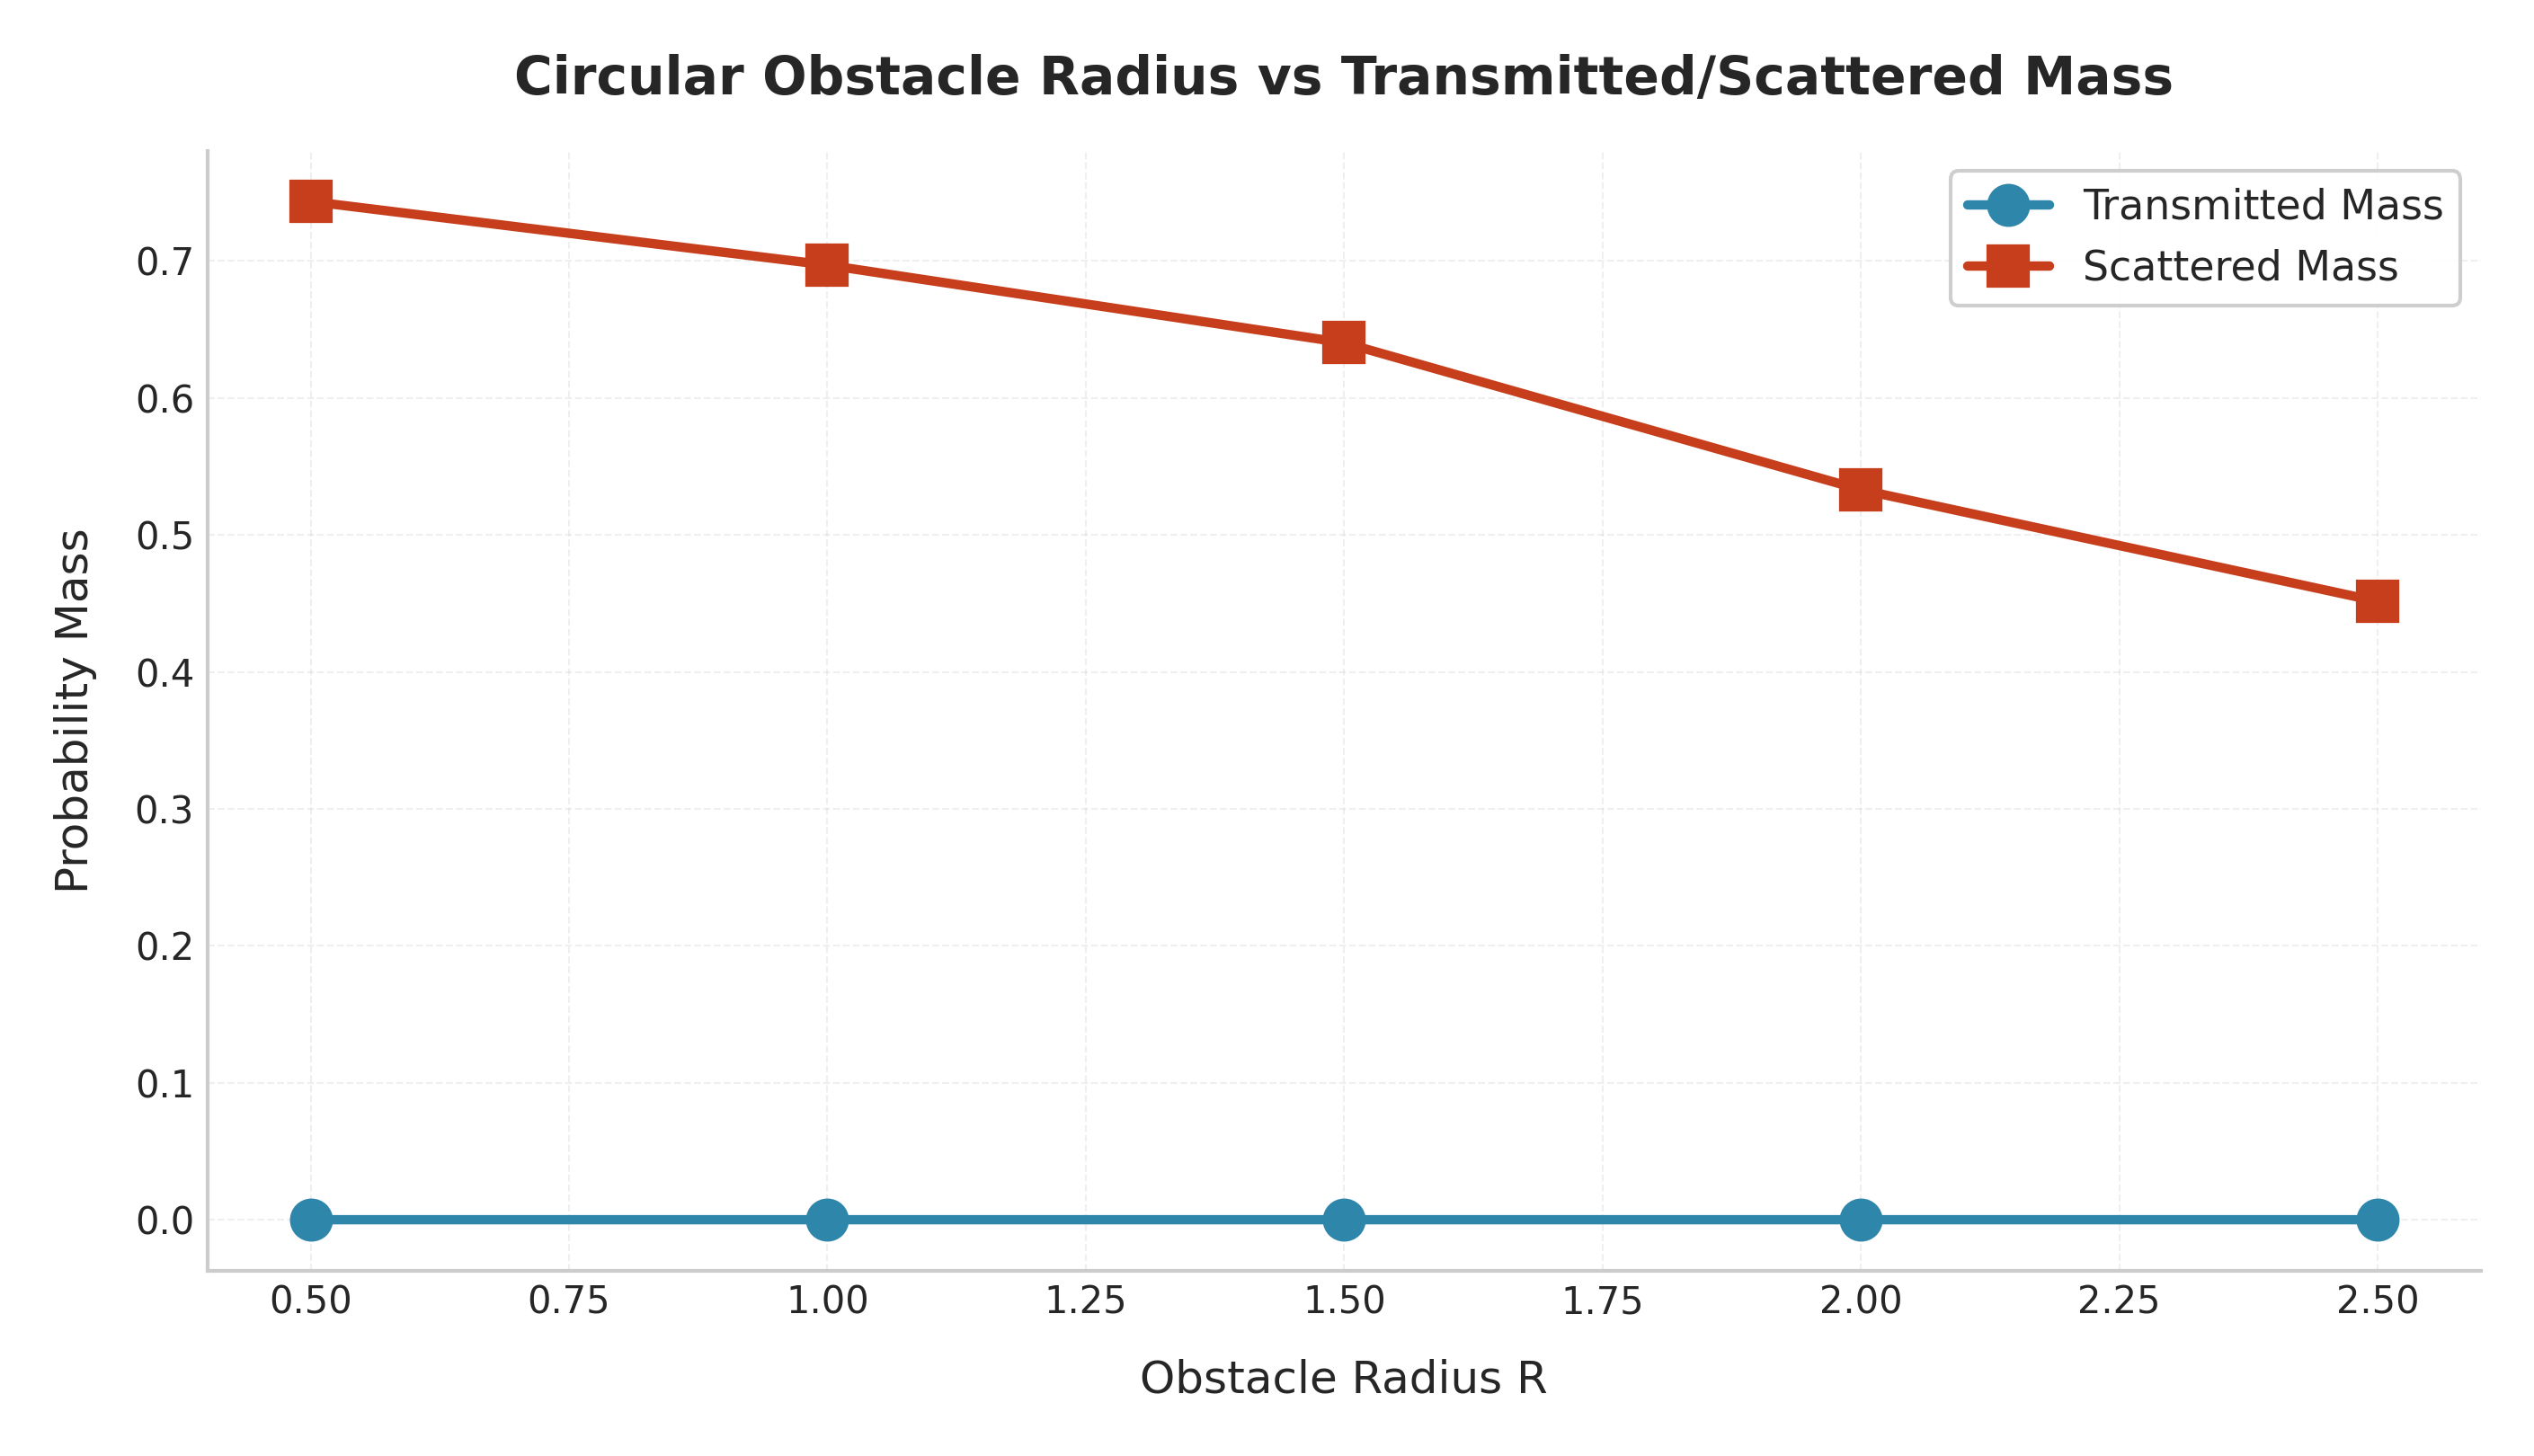
\includegraphics[width=0.70\textwidth]{figure_circular_sweep.png}
\caption{圆形障碍物半径参数扫描：透射质量与散射质量随半径 $R$ 的变化}
\label{fig:circular_sweep}
\end{figure}

\subsubsection{波导强度扫描}

图~\ref{fig:waveguide_sweep} 展示了波导强度 $\alpha$ 从 $0.1$ 到 $1.0$ 变化时，波束横向展宽（标准差 $\sigma_y$）的变化趋势。随着 $\alpha$ 增大，约束力增强，波束宽度显著减小——定量验证了波导强度的控制效果。

\begin{figure}[H]
\centering
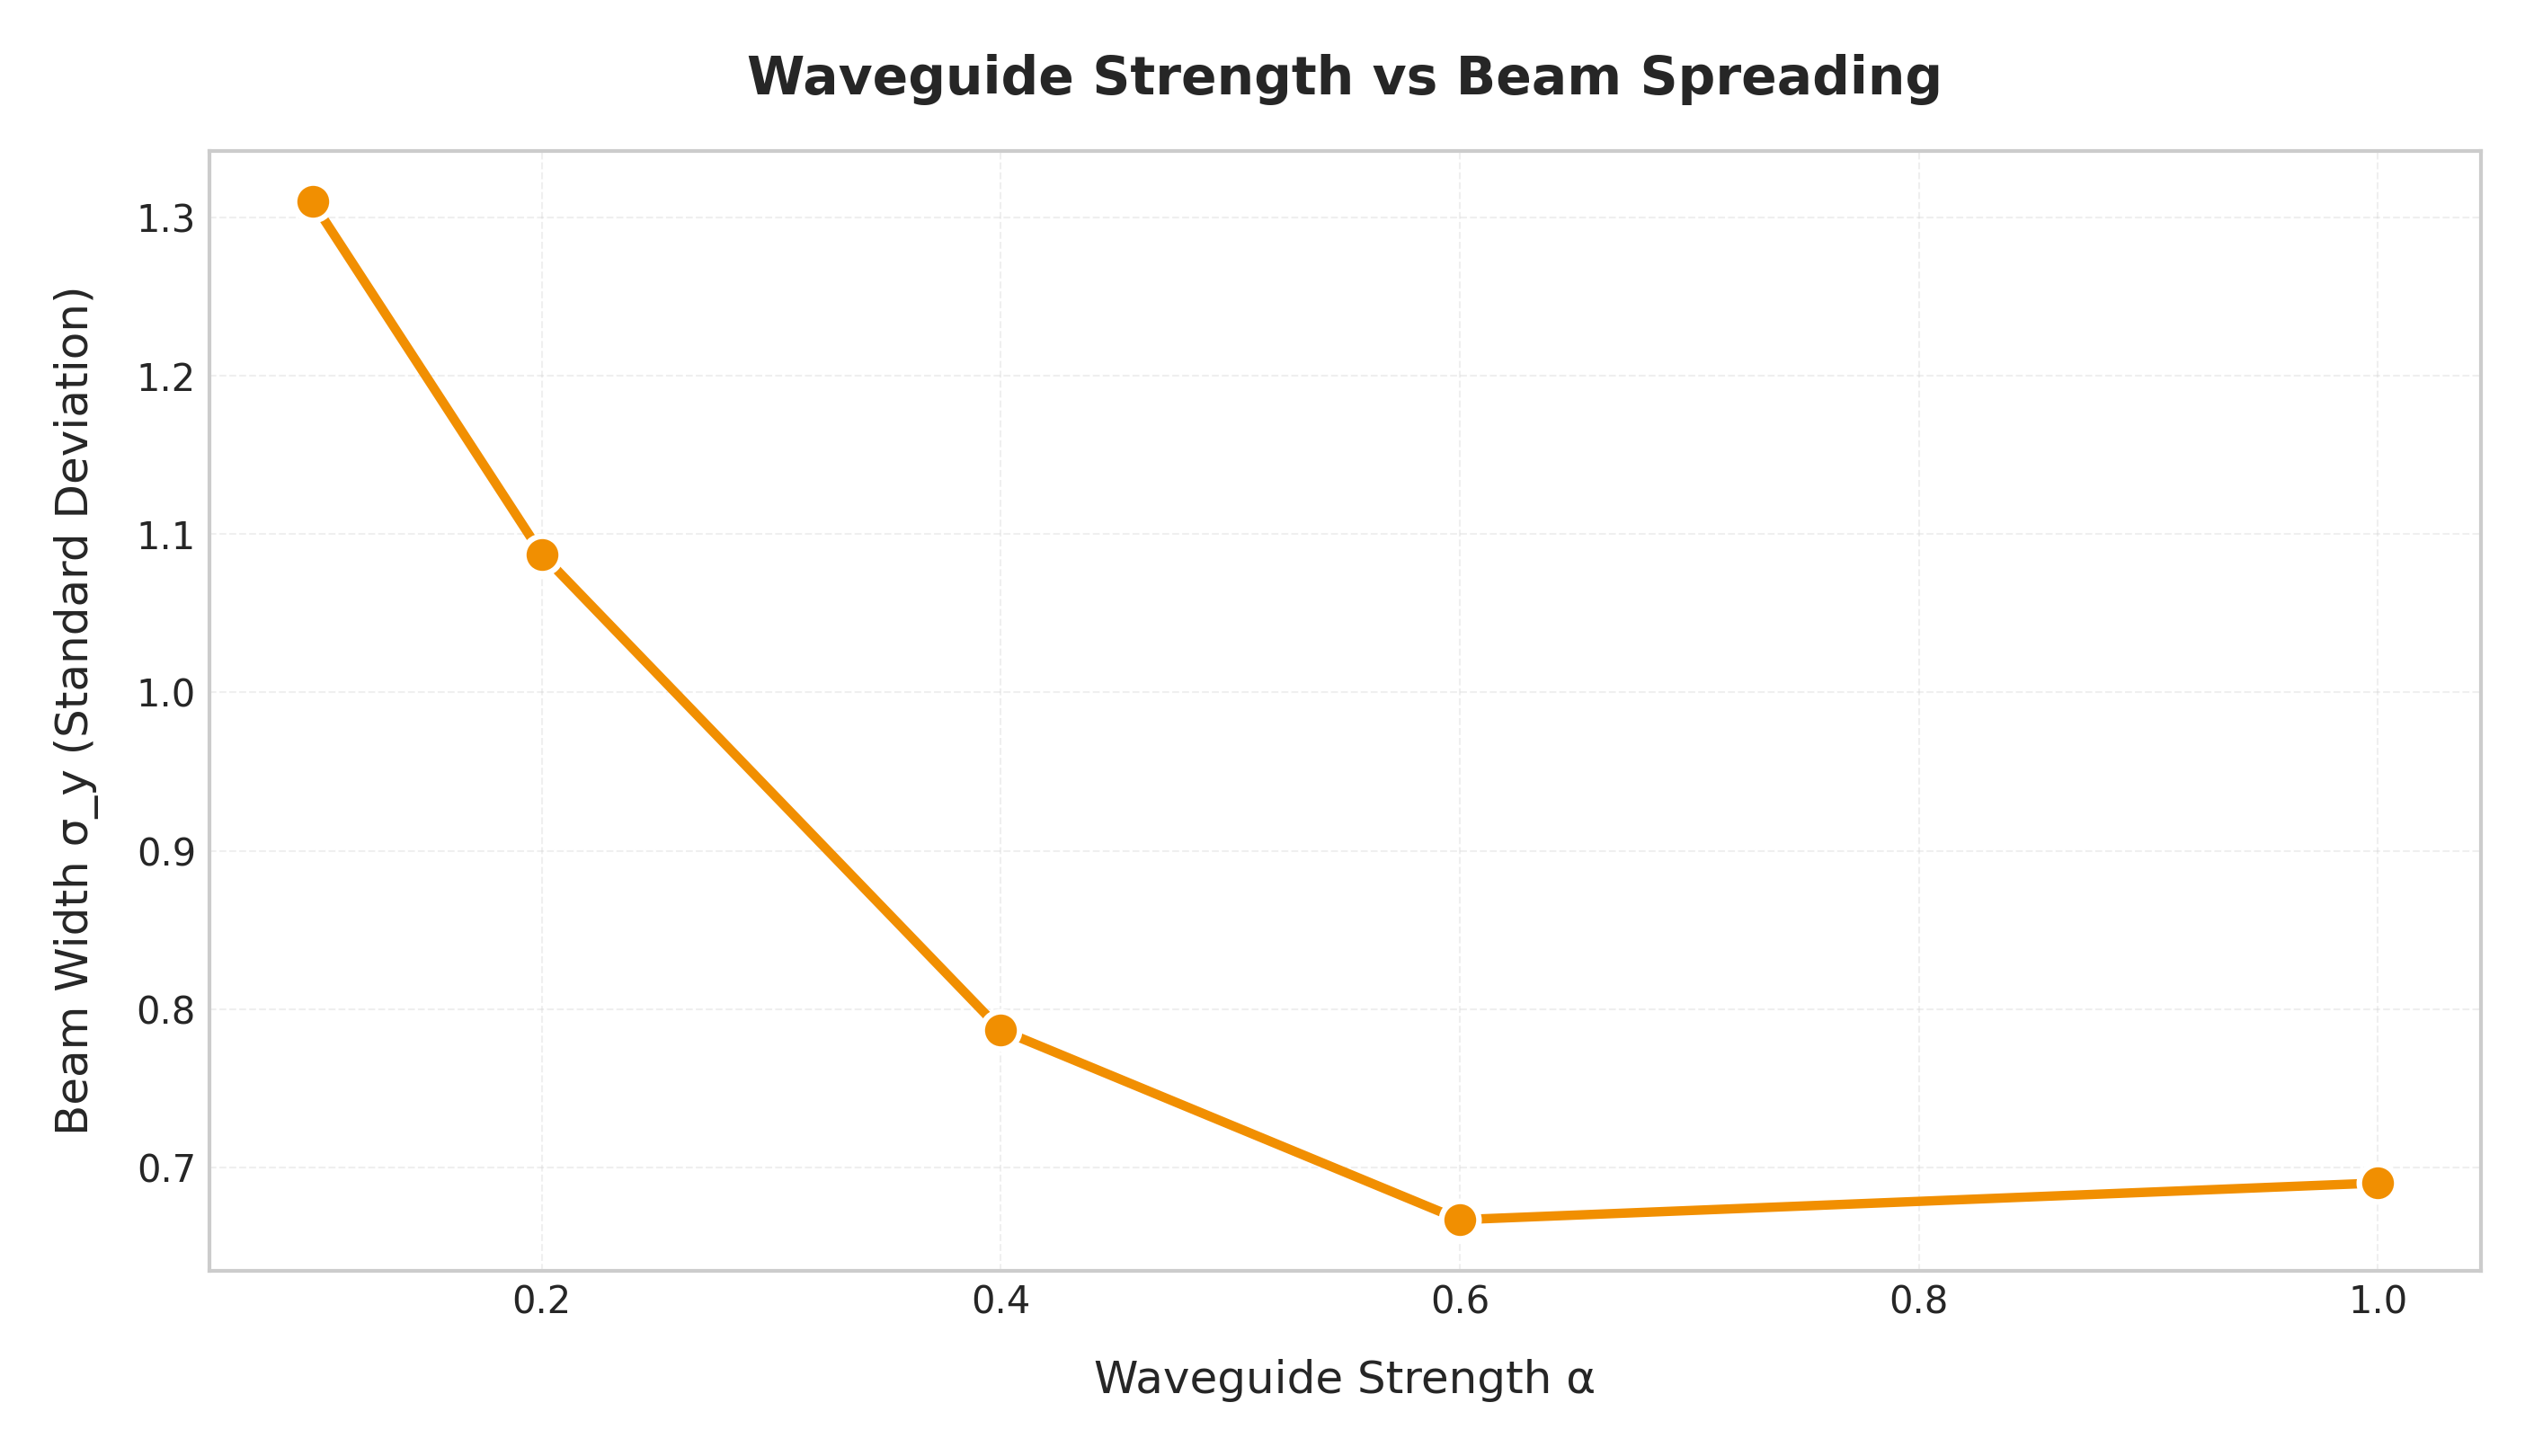
\includegraphics[width=0.70\textwidth]{figure_waveguide_sweep.png}
\caption{波导强度参数扫描：波束横向展宽 $\sigma_y$ 随波导强度 $\alpha$ 的变化}
\label{fig:waveguide_sweep}
\end{figure}

\subsection{二维收敛性与误差热图}

图~\ref{fig:2d_convergence} 展示了 Split-Step FFT 在二维自由高斯波包传播中的网格收敛性，包括 $L_1$/$L_2$/$L_\infty$ 误差随网格点数的对数-对数变化及其收敛阶数拟合，以及质量守恒误差在不同网格规模下的表现。

\begin{figure}[H]
\centering

\includegraphics[width=0.95\textwidth]{figure_2d_convergence.png}
\caption{二维收敛性分析：$L_1$/$L_2$/$L_\infty$ 误差随网格点数变化（左，双对数坐标）、质量守恒误差（中）、不同网格规模的质量对比（右）}
\label{fig:2d_convergence}
\end{figure}

图~\ref{fig:2d_error} 展示了二维数值解与精确解析解之间的逐点误差分布热图。上排为数值解与解析解的 $|\psi|^2$ 密度对比；下排为实部误差 $|\mathrm{Re}[\Delta\psi]|$ 和虚部误差 $|\mathrm{Im}[\Delta\psi]|$ 的分别展示。将复值误差分解为实部和虚部有助于判断误差的空间分布特征。

\begin{figure}[H]
\centering

\includegraphics[width=0.90\textwidth]{figure_2d_error_heatmap.png}
\caption{二维误差热图：数值解 $|\psi|^2$（左上）、解析解 $|\psi|^2$（右上）、实部误差 $|\mathrm{Re}[\Delta\psi]|$（左下）、虚部误差 $|\mathrm{Im}[\Delta\psi]|$（右下）}
\label{fig:2d_error}
\end{figure}

%==============================================================================
\section{代码架构}
%==============================================================================

本项目采用模块化 Python 包设计，代码组织如下：

\begin{itemize}
    \item \texttt{main.py} —— 主入口，提供命令行参数解析（\texttt{--quick}、\texttt{--no-gif}、\texttt{--exp}、\texttt{--dim}、\texttt{--list}、\texttt{--all} 等）和全部 18 个实验的调度执行。

    \item \texttt{tdse/experiments.py} —— 核心实验模块，包含全部预置实验函数：
    \begin{itemize}
        \item 一维核心实验（8 个）：解析对比、收敛性、稳定性、性能、动画、隧穿、方法对比、RTD 双势垒
        \item 二维实验（5 个）：自由传播、圆形障碍物散射、波导传播、ADI vs SSF 对比、误差热图、收敛性
        \item 分析实验（5 个）：质量守恒、运行时对比、全方法综合对比、圆形障碍物半径扫描、波导强度扫描
    \end{itemize}

    \item \texttt{tdse/solvers.py} —— 求解器模块：
    \begin{itemize}
        \item 五种一维格式的 step 函数：\texttt{step\_ftcs}、\texttt{step\_backward\_euler}、\texttt{step\_crank\_nicolson}、\texttt{step\_rk4}、\texttt{step\_split\_step\_fft}
        \item 二维方法：\texttt{step\_split\_step\_fft\_2d}、\texttt{step\_adi\_2d}
        \item 高层接口：\texttt{solve()}（1D）、\texttt{solve\_2d()}（2D）
        \item 求解器工厂类 \texttt{TDSESolverFactory} 和基类 \texttt{Solver1D}
    \end{itemize}

    \item \texttt{tdse/potentials.py} —— 势场与工具模块：
    \begin{itemize}
        \item 势场类体系：基类 \texttt{Potential1D}/\texttt{Potential2D}，具体势场类（Free、Harmonic、RectangularBarrier、DoubleBarrier1D、CircularObstacle、Waveguide）
        \item 势场工厂类 \texttt{TDSEPotentialFactory}
        \item 波函数初始化：\texttt{gaussian\_wavepacket}、\texttt{gaussian\_wavepacket\_2d}
        \item 解析解：\texttt{exact\_free\_gaussian}、\texttt{exact\_free\_gaussian\_2d}
        \item 本征态：\texttt{infinite\_well\_eigenstate}、\texttt{harmonic\_eigenstate\_low}
        \item 误差分析：\texttt{l1\_l2\_linf\_error}、\texttt{l2\_error\_real\_imag}（实/虚部分解）、\texttt{align\_global\_phase}
        \item 散射分析：\texttt{transmission\_reflection}、\texttt{compute\_transmission\_reflection}
        \item 网格生成：\texttt{grid}、\texttt{make\_2d\_grid}
    \end{itemize}

    \item \texttt{tdse/config.py} —— 配置模块：\texttt{RunConfig}/\texttt{TDSEConfig} 数据类，matplotlib 全局绘图样式设置。

    \item \texttt{tdse/visualization.py} —— 可视化模块：\texttt{TDSEVisualizer} 类（含三值视图方法 \texttt{plot\_complex\_comparison}），GIF 动画生成函数。

    \item \texttt{ex\_pinn.py} —— 物理信息神经网络（PINN）模块（可选，附录内容）。
\end{itemize}

以下代码片段展示了二维 ADI 方法的核心实现（\texttt{tdse/solvers.py} 中的 \texttt{step\_adi\_2d} 函数）：

\begin{lstlisting}[language=Python, caption={二维 ADI 方法核心实现（课本第~4章 CN 格式的二维推广）}, label={lst:adi}]
def step_adi_2d(psi, V, dx, dy, dt):
    # First half-step in x-direction
    for j in range(ny):
        # Build tridiagonal system for column j
        # (I + i*dt/2*H_x) psi_temp[:,j] = rhs
        psi_temp[:,j] = solve_banded((1,1), ab, rhs)

    # Full step in y-direction
    for i in range(nx):
        # (I + i*dt*H_y) psi_new[i,:] = rhs
        psi_new[i,:] = solve_banded((1,1), ab, rhs)

    # Second half-step in x-direction
    for j in range(ny):
        psi_new[:,j] = solve_banded((1,1), ab, rhs)

    return psi_new
\end{lstlisting}

%==============================================================================
\section{结论}
%==============================================================================

本文基于含时薛定谔方程（TDSE），对电子在一维和二维典型势场中的量子动力学行为进行了系统的数值模拟与分析。主要工作和结论如下：

\subsection{数值方法层面}

\begin{enumerate}
    \item 在一维情形下，五种数值格式的全面对比表明：
    \begin{itemize}
        \item \textbf{FTCS} 格式对 TDSE 条件不稳定，不应在实际计算中使用（但其发散行为有助于理解稳定性概念）。
        \item \textbf{Backward Euler} 格式无条件 $L_2$ 稳定但有数值耗散，不保持酉性，质量单调衰减。
        \item \textbf{Crank--Nicolson} 格式无条件稳定、二阶时间精度、保持酉性，是有限差分方法中的首选。
        \item \textbf{Split-Step FFT} 谱方法无条件稳定、保持酉性、具有谱空间精度，在大规模网格上效率最高。
        \item \textbf{RK4} 格式具有四阶时间精度但是条件稳定，适用性受限于时间步长的选取。
    \end{itemize}

    \item 在二维情形下，\textbf{ADI 方法}（课本第~4 章 CN 格式的二维推广）和 \textbf{Split-Step FFT} 方法各有优势：ADI 适用于非周期边界条件且无需 FFT；SSF 在周期边界下保持完美酉性和谱精度。两种方法的直接对比表明其精度处于同一量级（$L_2$ 差异 $\sim 10^{-4}$）。
\end{enumerate}

\subsection{物理模拟层面}

\begin{enumerate}
    \item \textbf{自由传播}：高斯波包的扩散和色散行为被所有稳定格式准确捕捉，与解析解高度吻合。
    \item \textbf{量子隧穿}：单势垒隧穿中透射系数随能量的变化符合量子力学预期；双势垒 RTD 结构中的共振隧穿效应被成功模拟——近共振时透射率接近 1。
    \item \textbf{波散射}：二维圆形障碍物散射清晰展示了前向散射为主的角分布特征。
    \item \textbf{约束传播}：二维波导有效地约束了波包的横向扩散，波导强度与束流宽度的定量关系被参数扫描实验验证。
\end{enumerate}

\subsection{分析方法层面：三值表示的创新价值}

本文系统性地采用了\textbf{复波函数的三重表示}（$|\psi|^2$、$\mathrm{Re}[\psi]$、$\mathrm{Im}[\psi]$）分析方法，其价值体现在：

\begin{itemize}
    \item \textbf{信息完整性}：$|\psi|^2$ 仅包含振幅信息，丢失了波函数的振荡符号和相位结构。实部和虚部共同编码了局部相位 $\phi = \arg\psi$，包含波前传播方向、波长、干涉图样等丰富信息。

    \item \textbf{物理洞察}：在量子隧穿（图~\ref{fig:1d_tunneling_reim}）和共振隧穿（图~\ref{fig:1d_rtd_reim}）实验中，实部和虚部清晰展示了 $|\psi|^2$ 无法揭示的驻波干涉图样和准束缚态振荡结构。

    \item \textbf{误差诊断}：通过实/虚部 $L_2$ 误差分解（综合对比实验，图~\ref{fig:all_methods}），可以判断数值格式的误差主导来源——非酉格式（Backward Euler）的实/虚部误差通常不均衡（系统性相位漂移），而酉格式（CN、SSF）在实部和虚部上具有一致的收敛行为。

    \item \textbf{相位可视化}：二维相位角热图（图~\ref{fig:2d_free_phase}）提供了波前结构的直观图像，是对密度热图的重要补充。
\end{itemize}

%==============================================================================
\appendix
\section{物理信息神经网络（PINN）方法}
%==============================================================================

作为传统数值方法的补充，本项目还实现了基于物理信息神经网络（Physics-Informed Neural Networks, PINN）的 1D TDSE 求解器（\texttt{ex\_pinn.py}）。PINN 将 PDE 残差作为损失函数的一部分，通过神经网络直接逼近波函数的实部和虚部：

\begin{equation}
    \psi(x,t) = u_\theta(x,t) + i\, v_\theta(x,t),
\end{equation}
其中 $u_\theta$ 和 $v_\theta$ 为全连接神经网络的输出。

损失函数由三部分组成：
\begin{align}
    \mathcal{L} &= \mathcal{L}_{\text{IC}} + \mathcal{L}_{\text{PDE}} + \mathcal{L}_{\text{BC}}, \\
    \mathcal{L}_{\text{IC}} &= \frac{1}{N_{\text{IC}}}\sum_{i} |\psi_\theta(x_i,0) - \psi_0(x_i)|^2, \\
    \mathcal{L}_{\text{PDE}} &= \frac{1}{N_r}\sum_{j} \left| i\frac{\partial\psi_\theta}{\partial t} + \frac{1}{2}\frac{\partial^2\psi_\theta}{\partial x^2} - V\psi_\theta \right|^2_{(x_j,t_j)}.
\end{align}

PINN 方法的特点在于无需网格离散化，直接将 PDE 编码为优化目标，但训练收敛速度较慢，精度目前不及传统数值方法。在全方法综合对比实验（图~\ref{fig:all_methods}）中，PINN 结果被包含在内供参考（需要 PyTorch 环境）。

\begin{thebibliography}{9}

\bibitem{leveque2007}
R.~J.~LeVeque, \textit{Finite Difference Methods for Ordinary and Partial Differential Equations: Steady-State and Time-Dependent Problems}, SIAM, 2007.

\bibitem{strang1968}
G.~Strang, ``On the construction and comparison of difference schemes,'' \textit{SIAM J. Numer. Anal.}, vol.~5, no.~3, pp.~506--517, 1968.

\bibitem{sulem1999}
C.~Sulem and P.~L.~Sulem, \textit{The Nonlinear Schr\"odinger Equation: Self-Focusing and Wave Collapse}, Springer, 1999.

\bibitem{raissi2019}
M.~Raissi, P.~Perdikaris, and G.~E.~Karniadakis, ``Physics-informed neural networks: A deep learning framework for solving forward and inverse problems involving nonlinear PDEs,'' \textit{J. Comput. Phys.}, vol.~378, pp.~686--707, 2019.

\bibitem{thijssen2007}
J.~M.~Thijssen, \textit{Computational Physics}, 2nd ed., Cambridge University Press, 2007.

\end{thebibliography}

\end{CJK}
\end{document}
